% Options for packages loaded elsewhere
\PassOptionsToPackage{unicode}{hyperref}
\PassOptionsToPackage{hyphens}{url}
\PassOptionsToPackage{dvipsnames,svgnames,x11names}{xcolor}
%
\documentclass[
  letterpaper,
  DIV=11,
  numbers=noendperiod]{scrreprt}

\usepackage{amsmath,amssymb}
\usepackage{iftex}
\ifPDFTeX
  \usepackage[T1]{fontenc}
  \usepackage[utf8]{inputenc}
  \usepackage{textcomp} % provide euro and other symbols
\else % if luatex or xetex
  \usepackage{unicode-math}
  \defaultfontfeatures{Scale=MatchLowercase}
  \defaultfontfeatures[\rmfamily]{Ligatures=TeX,Scale=1}
\fi
\usepackage{lmodern}
\ifPDFTeX\else  
    % xetex/luatex font selection
\fi
% Use upquote if available, for straight quotes in verbatim environments
\IfFileExists{upquote.sty}{\usepackage{upquote}}{}
\IfFileExists{microtype.sty}{% use microtype if available
  \usepackage[]{microtype}
  \UseMicrotypeSet[protrusion]{basicmath} % disable protrusion for tt fonts
}{}
\makeatletter
\@ifundefined{KOMAClassName}{% if non-KOMA class
  \IfFileExists{parskip.sty}{%
    \usepackage{parskip}
  }{% else
    \setlength{\parindent}{0pt}
    \setlength{\parskip}{6pt plus 2pt minus 1pt}}
}{% if KOMA class
  \KOMAoptions{parskip=half}}
\makeatother
\usepackage{xcolor}
\setlength{\emergencystretch}{3em} % prevent overfull lines
\setcounter{secnumdepth}{5}
% Make \paragraph and \subparagraph free-standing
\ifx\paragraph\undefined\else
  \let\oldparagraph\paragraph
  \renewcommand{\paragraph}[1]{\oldparagraph{#1}\mbox{}}
\fi
\ifx\subparagraph\undefined\else
  \let\oldsubparagraph\subparagraph
  \renewcommand{\subparagraph}[1]{\oldsubparagraph{#1}\mbox{}}
\fi

\usepackage{color}
\usepackage{fancyvrb}
\newcommand{\VerbBar}{|}
\newcommand{\VERB}{\Verb[commandchars=\\\{\}]}
\DefineVerbatimEnvironment{Highlighting}{Verbatim}{commandchars=\\\{\}}
% Add ',fontsize=\small' for more characters per line
\usepackage{framed}
\definecolor{shadecolor}{RGB}{241,243,245}
\newenvironment{Shaded}{\begin{snugshade}}{\end{snugshade}}
\newcommand{\AlertTok}[1]{\textcolor[rgb]{0.68,0.00,0.00}{#1}}
\newcommand{\AnnotationTok}[1]{\textcolor[rgb]{0.37,0.37,0.37}{#1}}
\newcommand{\AttributeTok}[1]{\textcolor[rgb]{0.40,0.45,0.13}{#1}}
\newcommand{\BaseNTok}[1]{\textcolor[rgb]{0.68,0.00,0.00}{#1}}
\newcommand{\BuiltInTok}[1]{\textcolor[rgb]{0.00,0.23,0.31}{#1}}
\newcommand{\CharTok}[1]{\textcolor[rgb]{0.13,0.47,0.30}{#1}}
\newcommand{\CommentTok}[1]{\textcolor[rgb]{0.37,0.37,0.37}{#1}}
\newcommand{\CommentVarTok}[1]{\textcolor[rgb]{0.37,0.37,0.37}{\textit{#1}}}
\newcommand{\ConstantTok}[1]{\textcolor[rgb]{0.56,0.35,0.01}{#1}}
\newcommand{\ControlFlowTok}[1]{\textcolor[rgb]{0.00,0.23,0.31}{#1}}
\newcommand{\DataTypeTok}[1]{\textcolor[rgb]{0.68,0.00,0.00}{#1}}
\newcommand{\DecValTok}[1]{\textcolor[rgb]{0.68,0.00,0.00}{#1}}
\newcommand{\DocumentationTok}[1]{\textcolor[rgb]{0.37,0.37,0.37}{\textit{#1}}}
\newcommand{\ErrorTok}[1]{\textcolor[rgb]{0.68,0.00,0.00}{#1}}
\newcommand{\ExtensionTok}[1]{\textcolor[rgb]{0.00,0.23,0.31}{#1}}
\newcommand{\FloatTok}[1]{\textcolor[rgb]{0.68,0.00,0.00}{#1}}
\newcommand{\FunctionTok}[1]{\textcolor[rgb]{0.28,0.35,0.67}{#1}}
\newcommand{\ImportTok}[1]{\textcolor[rgb]{0.00,0.46,0.62}{#1}}
\newcommand{\InformationTok}[1]{\textcolor[rgb]{0.37,0.37,0.37}{#1}}
\newcommand{\KeywordTok}[1]{\textcolor[rgb]{0.00,0.23,0.31}{#1}}
\newcommand{\NormalTok}[1]{\textcolor[rgb]{0.00,0.23,0.31}{#1}}
\newcommand{\OperatorTok}[1]{\textcolor[rgb]{0.37,0.37,0.37}{#1}}
\newcommand{\OtherTok}[1]{\textcolor[rgb]{0.00,0.23,0.31}{#1}}
\newcommand{\PreprocessorTok}[1]{\textcolor[rgb]{0.68,0.00,0.00}{#1}}
\newcommand{\RegionMarkerTok}[1]{\textcolor[rgb]{0.00,0.23,0.31}{#1}}
\newcommand{\SpecialCharTok}[1]{\textcolor[rgb]{0.37,0.37,0.37}{#1}}
\newcommand{\SpecialStringTok}[1]{\textcolor[rgb]{0.13,0.47,0.30}{#1}}
\newcommand{\StringTok}[1]{\textcolor[rgb]{0.13,0.47,0.30}{#1}}
\newcommand{\VariableTok}[1]{\textcolor[rgb]{0.07,0.07,0.07}{#1}}
\newcommand{\VerbatimStringTok}[1]{\textcolor[rgb]{0.13,0.47,0.30}{#1}}
\newcommand{\WarningTok}[1]{\textcolor[rgb]{0.37,0.37,0.37}{\textit{#1}}}

\providecommand{\tightlist}{%
  \setlength{\itemsep}{0pt}\setlength{\parskip}{0pt}}\usepackage{longtable,booktabs,array}
\usepackage{calc} % for calculating minipage widths
% Correct order of tables after \paragraph or \subparagraph
\usepackage{etoolbox}
\makeatletter
\patchcmd\longtable{\par}{\if@noskipsec\mbox{}\fi\par}{}{}
\makeatother
% Allow footnotes in longtable head/foot
\IfFileExists{footnotehyper.sty}{\usepackage{footnotehyper}}{\usepackage{footnote}}
\makesavenoteenv{longtable}
\usepackage{graphicx}
\makeatletter
\def\maxwidth{\ifdim\Gin@nat@width>\linewidth\linewidth\else\Gin@nat@width\fi}
\def\maxheight{\ifdim\Gin@nat@height>\textheight\textheight\else\Gin@nat@height\fi}
\makeatother
% Scale images if necessary, so that they will not overflow the page
% margins by default, and it is still possible to overwrite the defaults
% using explicit options in \includegraphics[width, height, ...]{}
\setkeys{Gin}{width=\maxwidth,height=\maxheight,keepaspectratio}
% Set default figure placement to htbp
\makeatletter
\def\fps@figure{htbp}
\makeatother

\usepackage{fvextra}
\DefineVerbatimEnvironment{Highlighting}{Verbatim}{breaklines,commandchars=\\\{\}}
\DefineVerbatimEnvironment{OutputCode}{Verbatim}{breaklines,commandchars=\\\{\}}
\KOMAoption{captions}{tableheading}
\makeatletter
\@ifpackageloaded{tcolorbox}{}{\usepackage[skins,breakable]{tcolorbox}}
\@ifpackageloaded{fontawesome5}{}{\usepackage{fontawesome5}}
\definecolor{quarto-callout-color}{HTML}{909090}
\definecolor{quarto-callout-note-color}{HTML}{0758E5}
\definecolor{quarto-callout-important-color}{HTML}{CC1914}
\definecolor{quarto-callout-warning-color}{HTML}{EB9113}
\definecolor{quarto-callout-tip-color}{HTML}{00A047}
\definecolor{quarto-callout-caution-color}{HTML}{FC5300}
\definecolor{quarto-callout-color-frame}{HTML}{acacac}
\definecolor{quarto-callout-note-color-frame}{HTML}{4582ec}
\definecolor{quarto-callout-important-color-frame}{HTML}{d9534f}
\definecolor{quarto-callout-warning-color-frame}{HTML}{f0ad4e}
\definecolor{quarto-callout-tip-color-frame}{HTML}{02b875}
\definecolor{quarto-callout-caution-color-frame}{HTML}{fd7e14}
\makeatother
\makeatletter
\makeatother
\makeatletter
\@ifpackageloaded{bookmark}{}{\usepackage{bookmark}}
\makeatother
\makeatletter
\@ifpackageloaded{caption}{}{\usepackage{caption}}
\AtBeginDocument{%
\ifdefined\contentsname
  \renewcommand*\contentsname{Table of contents}
\else
  \newcommand\contentsname{Table of contents}
\fi
\ifdefined\listfigurename
  \renewcommand*\listfigurename{List of Figures}
\else
  \newcommand\listfigurename{List of Figures}
\fi
\ifdefined\listtablename
  \renewcommand*\listtablename{List of Tables}
\else
  \newcommand\listtablename{List of Tables}
\fi
\ifdefined\figurename
  \renewcommand*\figurename{Figure}
\else
  \newcommand\figurename{Figure}
\fi
\ifdefined\tablename
  \renewcommand*\tablename{Table}
\else
  \newcommand\tablename{Table}
\fi
}
\@ifpackageloaded{float}{}{\usepackage{float}}
\floatstyle{ruled}
\@ifundefined{c@chapter}{\newfloat{codelisting}{h}{lop}}{\newfloat{codelisting}{h}{lop}[chapter]}
\floatname{codelisting}{Listing}
\newcommand*\listoflistings{\listof{codelisting}{List of Listings}}
\makeatother
\makeatletter
\@ifpackageloaded{caption}{}{\usepackage{caption}}
\@ifpackageloaded{subcaption}{}{\usepackage{subcaption}}
\makeatother
\makeatletter
\@ifpackageloaded{tcolorbox}{}{\usepackage[skins,breakable]{tcolorbox}}
\makeatother
\makeatletter
\@ifundefined{shadecolor}{\definecolor{shadecolor}{rgb}{.97, .97, .97}}
\makeatother
\makeatletter
\makeatother
\makeatletter
\makeatother
\ifLuaTeX
  \usepackage{selnolig}  % disable illegal ligatures
\fi
\IfFileExists{bookmark.sty}{\usepackage{bookmark}}{\usepackage{hyperref}}
\IfFileExists{xurl.sty}{\usepackage{xurl}}{} % add URL line breaks if available
\urlstyle{same} % disable monospaced font for URLs
\hypersetup{
  pdftitle={GEOG0114 Principles of Spatial Analysis},
  pdfauthor={Justin van Dijk},
  colorlinks=true,
  linkcolor={blue},
  filecolor={Maroon},
  citecolor={Blue},
  urlcolor={Blue},
  pdfcreator={LaTeX via pandoc}}

\title{GEOG0114 Principles of Spatial Analysis}
\author{Justin van Dijk}
\date{2023-09-22}

\begin{document}
\maketitle
\ifdefined\Shaded\renewenvironment{Shaded}{\begin{tcolorbox}[enhanced, interior hidden, breakable, frame hidden, boxrule=0pt, sharp corners, borderline west={3pt}{0pt}{shadecolor}]}{\end{tcolorbox}}\fi

\renewcommand*\contentsname{Table of contents}
{
\hypersetup{linkcolor=}
\setcounter{tocdepth}{2}
\tableofcontents
}
\bookmarksetup{startatroot}

\hypertarget{module-overview}{%
\chapter*{Module overview}\label{module-overview}}
\addcontentsline{toc}{chapter}{Module overview}

\markboth{Module overview}{Module overview}


\includegraphics[width=1\textwidth,height=\textheight]{images/w00/data-science-welcome-sm.jpg}

\begin{longtable}[]{@{}
  >{\raggedright\arraybackslash}p{(\columnwidth - 4\tabcolsep) * \real{0.0857}}
  >{\raggedright\arraybackslash}p{(\columnwidth - 4\tabcolsep) * \real{0.3714}}
  >{\raggedright\arraybackslash}p{(\columnwidth - 4\tabcolsep) * \real{0.5429}}@{}}
\toprule\noalign{}
\begin{minipage}[b]{\linewidth}\raggedright
Week
\end{minipage} & \begin{minipage}[b]{\linewidth}\raggedright
Section
\end{minipage} & \begin{minipage}[b]{\linewidth}\raggedright
Topic
\end{minipage} \\
\midrule\noalign{}
\endhead
\bottomrule\noalign{}
\endlastfoot
1 & Foundational Concepts &
\href{https://uclpg-msc-sgds.github.io/GEOG0114}{Spatial analysis for
data science} \\
2 & Foundational Concepts &
\href{https://uclpg-msc-sgds.github.io/GEOG0114}{Graphical
representation of spatial data} \\
3 & Foundational Concepts &
\href{https://uclpg-msc-sgds.github.io/GEOG0114}{Spatial
autocorrelation} \\
4 & Raster data &
\href{https://uclpg-msc-sgds.github.io/GEOG0114}{Suitability Mapping
I} \\
5 & Raster data &
\href{https://uclpg-msc-sgds.github.io/GEOG0114}{Suitability Mapping
II} \\
& \textbf{Reading week} & \textbf{Reading week} \\
6 & Raster data &
\href{https://uclpg-msc-sgds.github.io/GEOG0114}{Geostatistics using
Kriging} \\
7 & Applied Spatial Analysis &
\href{01-geodemographics.html}{Geodemographics} \\
8 & Applied Spatial Analysis & \href{02-network.html}{Transport network
analysis} \\
9 & Spatial models &
\href{https://uclpg-msc-sgds.github.io/GEOG0114}{Spatial models I} \\
10 & Spatial models &
\href{https://uclpg-msc-sgds.github.io/GEOG0114}{Spatial models II} \\
\end{longtable}

\begin{tcolorbox}[enhanced jigsaw, rightrule=.15mm, colback=white, opacityback=0, opacitybacktitle=0.6, coltitle=black, colbacktitle=quarto-callout-note-color!10!white, breakable, arc=.35mm, title=\textcolor{quarto-callout-note-color}{\faInfo}\hspace{0.5em}{Note}, left=2mm, leftrule=.75mm, bottomtitle=1mm, toprule=.15mm, bottomrule=.15mm, colframe=quarto-callout-note-color-frame, toptitle=1mm, titlerule=0mm]

This GitHub page contains the material for Week 07
(\href{01-geodemographics.html}{Geodemographics}) and Week 08
(\href{02-transport-network-analysis.html}{Transport network analysis})
of \textbf{Principles of Spatial Analysis} 2023-2024. The content for
2022-2023 has been archived and can be found here:
\href{https://jtvandijk.github.io/GEOG0114_20222023}{{[}Link{]}}

\end{tcolorbox}

\bookmarksetup{startatroot}

\hypertarget{geodemographics}{%
\chapter{Geodemographics}\label{geodemographics}}

This week we will see how we can use socio-demographic and
socio-economic data to characterise neighbourhoods using
\textbf{geodemographics}. Geodemographics is the ``\emph{analysis of
people by where they live (Harris et al.~2005) and as such entails
representing the individual and collective identities that are manifest
in observable neighbourhood structure}''
(\href{https://doi.org/10.1080/13658816.2012.719623}{Longley 2012}). We
will look at geodemographics by focusing on an existing geodemographic
classification known as the
\href{https://data.cdrc.ac.uk/dataset/internet-user-classification}{Internet
User Classification}.

\hypertarget{lecture-w07}{%
\section{Lecture slides}\label{lecture-w07}}

You can download the slides of this week's lecture here:
\href{https://github.com/jtvandijk/GEOG0114Q/tree/master/slides/w07-psa.pdf}{{[}Link{]}}.

\hypertarget{reading-w07}{%
\section{Reading list}\label{reading-w07}}

\hypertarget{essential-readings}{%
\subsubsection*{Essential readings}\label{essential-readings}}
\addcontentsline{toc}{subsubsection}{Essential readings}

\begin{itemize}
\tightlist
\item
  Longley, P. A. 2012. Geodemographics and the practices of geographic
  information science. \emph{International Journal of Geographical
  Information Science} 26(12): 2227-2237.
  \href{https://doi.org/10.1080/13658816.2012.719623}{{[}Link{]}}
\item
  Martin, D., Gale, C., Cockings, S. \emph{et al.} 2018.
  Origin-destination geodemographics for analysis of travel to work
  flows. \emph{Computers, Environment and Urban Systems} 67: 68-79.
  \href{https://doi.org/10.1016/j.compenvurbsys.2017.09.002}{{[}Link{]}}
\item
  Singleton, A., Alexiou, A. and Savani, R. 2020. Mapping the
  geodemographics of digital inequality in Great Britain: An integration
  of machine learning into small area estimation. \emph{Computers,
  Environment and Urban Systems} 82: 101486.
  \href{https://doi.org/10.1016/j.compenvurbsys.2020.101486}{{[}Link{]}}
\item
  Singleton, A. and Spielman, S. 2014. The past, present, and future of
  geodemographic research in the United States and United Kingdom.
  \emph{The Professional Geographer} 66(4): 558-567.
  \href{https://doi.org/10.1080/00330124.2013.848764}{{[}Link{]}}
\end{itemize}

\hypertarget{suggested-readings}{%
\subsubsection*{Suggested readings}\label{suggested-readings}}
\addcontentsline{toc}{subsubsection}{Suggested readings}

\begin{itemize}
\tightlist
\item
  Goodman, A., Wilkinson, P., Stafford, M. \emph{et al.} 2011.
  Characterising socio-economic inequalities in exposure to air
  pollution: A comparison of socio-economic markers and scales of
  measurement. \emph{Health \& Place} 17(3): 767-774.
  \href{https://doi.org/10.1016/j.healthplace.2011.02.002}{{[}Link{]}}
\end{itemize}

\hypertarget{geodemographics-1}{%
\section{Geodemographics}\label{geodemographics-1}}

The
\href{https://data.cdrc.ac.uk/dataset/internet-user-classification}{CDRC
Internet User Classification} (IUC) is a bespoke geodemographic
classification that describes how people residing in different parts of
Great Britain interact with the Internet. For every Lower Super Output
Area (LSOA) in England and Wales and Data Zone (DZ)
(\href{https://www.ons.gov.uk/methodology/geography/ukgeographies/censusgeography}{2011
Census Geographies}), the IUC provides aggregate population estimates of
Internet use and provides insights into the geography of the digital
divide in the United Kingdom:

\begin{quote}
``Digital inequality is observable where access to online resources and
those opportunities that these create are non-egalitarian. As a result
of variable rates of access and use of the Internet between social and
spatial groups (..), this leads to digital differentiation, which
entrenches difference and reciprocates digital inequality over time''
(\href{https://doi.org/10.1016/j.compenvurbsys.2020.101486}{Singleton
\emph{et al.} 2020}).
\end{quote}

\hypertarget{internet-user-classification-i}{%
\subsection{Internet User Classification
I}\label{internet-user-classification-i}}

For the first part of this week's practical material, we will be looking
at the Internet User Classification (IUC) for Great Britain in more
detail by mapping it.

Our first step is to download the IUC data set:

\begin{itemize}
\tightlist
\item
  Open a web browser and go to the \href{https://data.cdrc.ac.uk}{data
  portal of the CDRC}.
\item
  Register if you need to, or if you are already registered, make sure
  you are logged in.
\item
  Search for \textbf{Internet User Classification}.
\item
  Scroll down and choose the download option for the \emph{IUC 2018
  (CSV)}.
\item
  Save the \texttt{iuc\_gb\_2018.csv} file in an appropriate folder.
\end{itemize}

\begin{figure}

{\centering 
\includegraphics[width=1\textwidth,height=\textheight]{images/w07/iuc-download.png}

}

\caption{\label{fig-geo-iuc-download}Download the GB IUC 2018}

\end{figure}

Start by inspecting the data set in MS Excel, or any other spreadsheet
software such as
\href{https://www.openoffice.org/product/calc.html}{Apache OpenOffice
Calc} or \href{https://www.apple.com/uk/numbers/}{Numbers}. Also, have a
look at the
\href{https://data.cdrc.ac.uk/system/files/iuc2018userguide.pdf}{IUC
2018 User Guide} that provides the \textbf{pen portraits} of every
cluster, including plots of cluster centres and a brief summary of the
methodology.

\begin{tcolorbox}[enhanced jigsaw, rightrule=.15mm, colback=white, opacityback=0, opacitybacktitle=0.6, coltitle=black, colbacktitle=quarto-callout-tip-color!10!white, breakable, arc=.35mm, title=\textcolor{quarto-callout-tip-color}{\faLightbulb}\hspace{0.5em}{Tip}, left=2mm, leftrule=.75mm, bottomtitle=1mm, toprule=.15mm, bottomrule=.15mm, colframe=quarto-callout-tip-color-frame, toptitle=1mm, titlerule=0mm]

It is always a good idea to inspect your data prior to analysis to find
out how your data look like. Of course, depending on the type of data,
you can choose any tool you like to do this inspection
(\href{https://www.arcgis.com/index.html}{ArcGIS},
\href{https://www.r-project.org/}{R},
\href{https://qgis.org/en/site/}{QGIS},
\href{https://www.office.com/}{Microsoft Excel}, etc.).

\end{tcolorbox}

\begin{figure}

{\centering 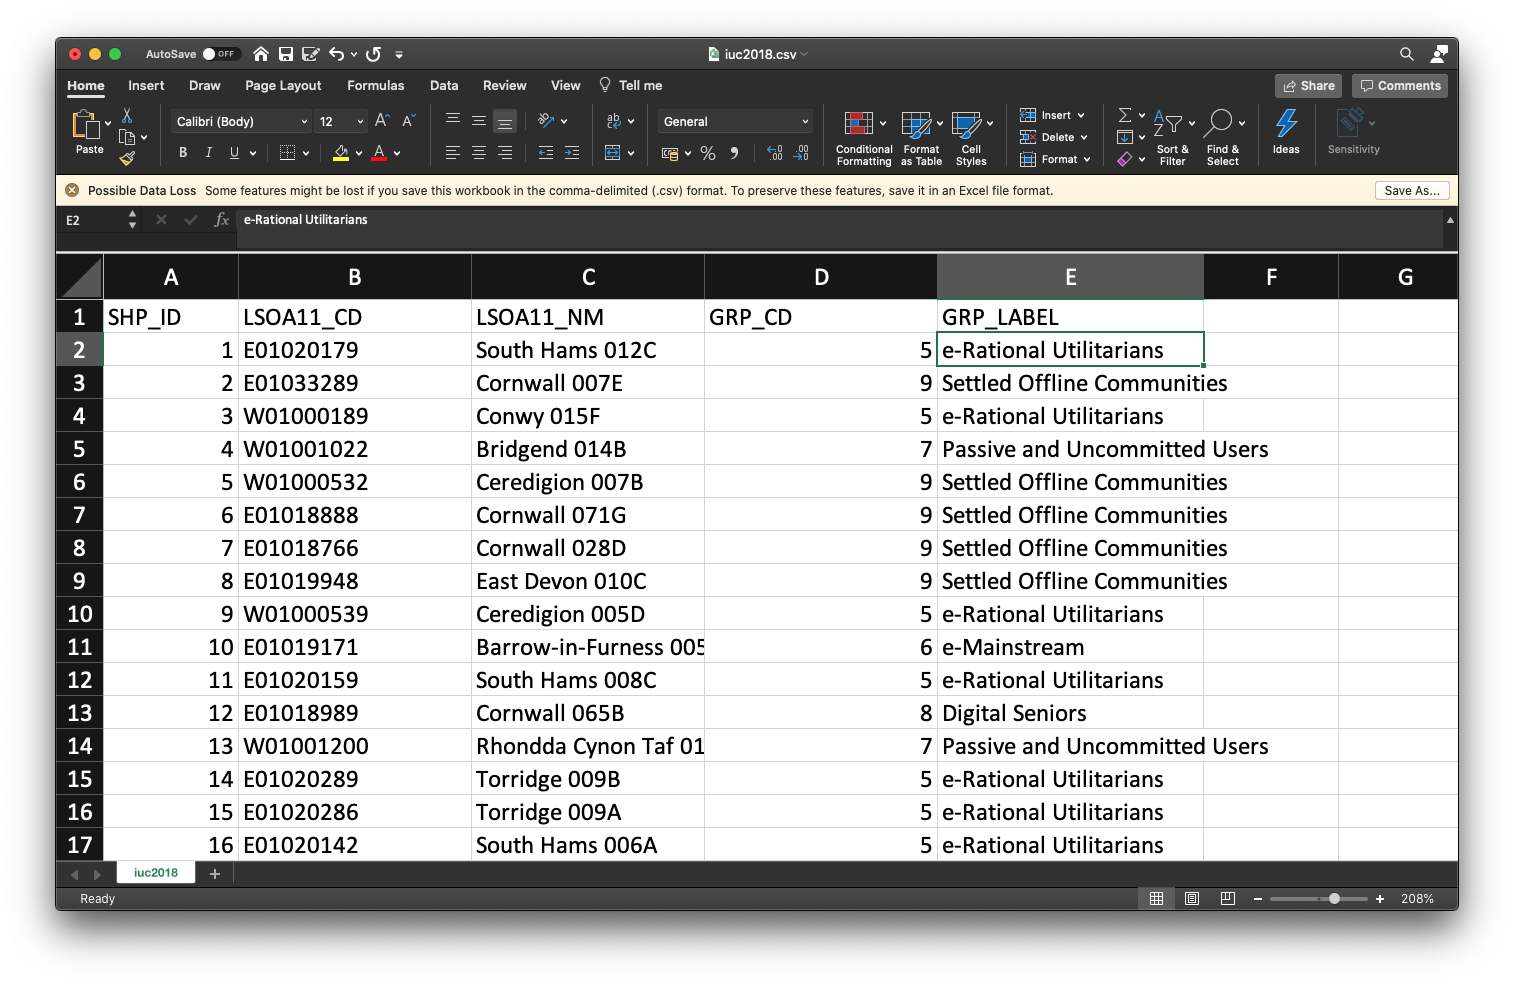
\includegraphics[width=1\textwidth,height=\textheight]{images/w07/iuc-excel.png}

}

\caption{\label{fig-geo-iuc-in-excel}GB IUC 2018 in Excel}

\end{figure}

\begin{codelisting}

\caption{\texttt{R code}}

\begin{Shaded}
\begin{Highlighting}[]
\CommentTok{\# load libraries}
\FunctionTok{library}\NormalTok{(tidyverse)}
\FunctionTok{library}\NormalTok{(tmap)}

\CommentTok{\# load data}
\NormalTok{iuc }\OtherTok{\textless{}{-}} \FunctionTok{read\_csv}\NormalTok{(}\StringTok{"data/index/iuc{-}gb{-}2018.csv"}\NormalTok{)}

\CommentTok{\# inspect}
\NormalTok{iuc}
\end{Highlighting}
\end{Shaded}

\end{codelisting}

\begin{verbatim}
# A tibble: 41,729 x 5
   SHP_ID LSOA11_CD LSOA11_NM              GRP_CD GRP_LABEL                    
    <dbl> <chr>     <chr>                   <dbl> <chr>                        
 1      1 E01020179 South Hams 012C             5 e-Rational Utilitarians      
 2      2 E01033289 Cornwall 007E               9 Settled Offline Communities  
 3      3 W01000189 Conwy 015F                  5 e-Rational Utilitarians      
 4      4 W01001022 Bridgend 014B               7 Passive and Uncommitted Users
 5      5 W01000532 Ceredigion 007B             9 Settled Offline Communities  
 6      6 E01018888 Cornwall 071G               9 Settled Offline Communities  
 7      7 E01018766 Cornwall 028D               9 Settled Offline Communities  
 8      8 E01019948 East Devon 010C             9 Settled Offline Communities  
 9      9 W01000539 Ceredigion 005D             5 e-Rational Utilitarians      
10     10 E01019171 Barrow-in-Furness 005E      6 e-Mainstream                 
# ... with 41,719 more rows
\end{verbatim}

\begin{codelisting}

\caption{\texttt{R code}}

\begin{Shaded}
\begin{Highlighting}[]
\CommentTok{\# inspect data types}
\FunctionTok{str}\NormalTok{(iuc)}
\end{Highlighting}
\end{Shaded}

\end{codelisting}

\begin{verbatim}
spc_tbl_ [41,729 x 5] (S3: spec_tbl_df/tbl_df/tbl/data.frame)
 $ SHP_ID   : num [1:41729] 1 2 3 4 5 6 7 8 9 10 ...
 $ LSOA11_CD: chr [1:41729] "E01020179" "E01033289" "W01000189" "W01001022" ...
 $ LSOA11_NM: chr [1:41729] "South Hams 012C" "Cornwall 007E" "Conwy 015F" "Bridgend 014B" ...
 $ GRP_CD   : num [1:41729] 5 9 5 7 9 9 9 9 5 6 ...
 $ GRP_LABEL: chr [1:41729] "e-Rational Utilitarians" "Settled Offline Communities" "e-Rational Utilitarians" "Passive and Uncommitted Users" ...
 - attr(*, "spec")=
  .. cols(
  ..   SHP_ID = col_double(),
  ..   LSOA11_CD = col_character(),
  ..   LSOA11_NM = col_character(),
  ..   GRP_CD = col_double(),
  ..   GRP_LABEL = col_character()
  .. )
 - attr(*, "problems")=<externalptr> 
\end{verbatim}

Now the data are loaded we can move to acquiring our spatial data. As
the IUC is created at the level of the Lower layer Super Output Area
\href{https://www.ons.gov.uk/methodology/geography/ukgeographies/censusgeography}{Census
geography}, we need to download its administrative borders. As the data
set for the entire country is quite large, we will focus on
\href{https://en.wikipedia.org/wiki/Liverpool}{Liverpool}.

\begin{itemize}
\tightlist
\item
  Go to the \href{https://borders.ukdataservice.ac.uk/}{UK Data Service
  Census support portal} and select \textbf{Boundary Data Selector}.
\item
  Set Country to \emph{England}, Geography to \emph{Statistical Building
  Block}, dates to \emph{2011 and later}, and click \textbf{Find}.
\item
  Select \emph{English Lower Layer Super Output Areas, 2011} and click
  \textbf{List Areas}.
\item
  Select \emph{Liverpool} from the list and click \textbf{Extract
  Boundary Data}.
\item
  Wait until loaded and download the \texttt{BoundaryData.zip} file.
\item
  Unzip and save the file.
\end{itemize}

\begin{tcolorbox}[enhanced jigsaw, rightrule=.15mm, colback=white, opacityback=0, opacitybacktitle=0.6, coltitle=black, colbacktitle=quarto-callout-note-color!10!white, breakable, arc=.35mm, title=\textcolor{quarto-callout-note-color}{\faInfo}\hspace{0.5em}{Note}, left=2mm, leftrule=.75mm, bottomtitle=1mm, toprule=.15mm, bottomrule=.15mm, colframe=quarto-callout-note-color-frame, toptitle=1mm, titlerule=0mm]

You could also have downloaded the shapefile with the data already
joined to the LSOA boundaries directly from the CDRC data portal, but
this is the national data set and is quite large (75MB). Also, as we
will be looking at
\href{https://en.wikipedia.org/wiki/Liverpool}{Liverpool} today we do
not need all LSOAs in Great Britain..

\end{tcolorbox}

Now we got the administrative boundary data, we can prepare the IUC map
by joining our \texttt{csv} file with the IUC classification to the
\texttt{shapefile}.

\begin{codelisting}

\caption{\texttt{R code}}

\begin{Shaded}
\begin{Highlighting}[]
\CommentTok{\# load libraries}
\FunctionTok{library}\NormalTok{(sf)}
\FunctionTok{library}\NormalTok{(tmap)}

\CommentTok{\# load spatial data}
\NormalTok{liverpool }\OtherTok{\textless{}{-}} \FunctionTok{st\_read}\NormalTok{(}\StringTok{"data/boundaries/england\_lsoa\_2011.shp"}\NormalTok{)}
\end{Highlighting}
\end{Shaded}

\end{codelisting}

\begin{verbatim}
Reading layer `england_lsoa_2011' from data source 
  `/Users/justinvandijk/Library/CloudStorage/Dropbox/UCL/Web/jtvandijk.github.io/GEOG0114Q/data/boundaries/england_lsoa_2011.shp' 
  using driver `ESRI Shapefile'
Simple feature collection with 298 features and 3 fields
Geometry type: POLYGON
Dimension:     XY
Bounding box:  xmin: 332390.2 ymin: 379748.5 xmax: 345636 ymax: 397980.1
Projected CRS: OSGB36 / British National Grid
\end{verbatim}

\begin{Shaded}
\begin{Highlighting}[]
\CommentTok{\# inspect}
\FunctionTok{tm\_shape}\NormalTok{(liverpool) }\SpecialCharTok{+} \FunctionTok{tm\_polygons}\NormalTok{()}
\end{Highlighting}
\end{Shaded}

\begin{figure}[H]

{\centering 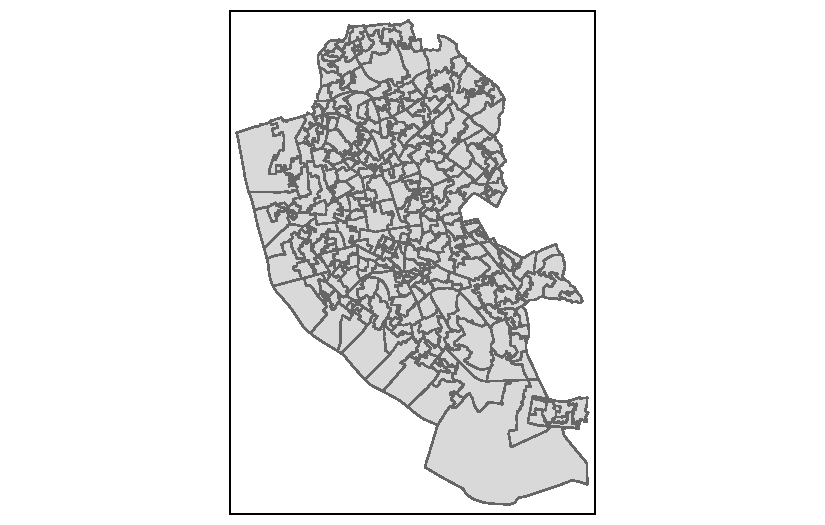
\includegraphics{01-geodemographics_files/figure-pdf/fig-geo-load-those-spatial-data-1.pdf}

}

\caption{\label{fig-geo-load-those-spatial-data}LSOAs Liverpool}

\end{figure}

\begin{codelisting}

\caption{\texttt{R code}}

\begin{Shaded}
\begin{Highlighting}[]
\CommentTok{\# join data}
\NormalTok{liv\_iuc }\OtherTok{\textless{}{-}} \FunctionTok{left\_join}\NormalTok{(liverpool, iuc, }\AttributeTok{by =} \FunctionTok{c}\NormalTok{(}\AttributeTok{code =} \StringTok{"LSOA11\_CD"}\NormalTok{))}

\CommentTok{\# inspect}
\NormalTok{liv\_iuc}
\end{Highlighting}
\end{Shaded}

\end{codelisting}

\begin{verbatim}
Simple feature collection with 298 features and 7 fields
Geometry type: POLYGON
Dimension:     XY
Bounding box:  xmin: 332390.2 ymin: 379748.5 xmax: 345636 ymax: 397980.1
Projected CRS: OSGB36 / British National Grid
First 10 features:
                         label           name      code SHP_ID      LSOA11_NM
1  E08000012E02006934E01033755 Liverpool 062D E01033755  25097 Liverpool 062D
2  E08000012E02006932E01033758 Liverpool 060B E01033758  24070 Liverpool 060B
3  E08000012E02001356E01033759 Liverpool 010F E01033759  26845 Liverpool 010F
4  E08000012E02006932E01033762 Liverpool 060E E01033762  26866 Liverpool 060E
5  E08000012E02001396E01032505 Liverpool 050F E01032505  27848 Liverpool 050F
6  E08000012E02001396E01032506 Liverpool 050G E01032506   2429 Liverpool 050G
7  E08000012E02001396E01032507 Liverpool 050H E01032507  24242 Liverpool 050H
8  E08000012E02001373E01032508 Liverpool 027G E01032508  28413 Liverpool 027G
9  E08000012E02001373E01032509 Liverpool 027H E01032509  24339 Liverpool 027H
10 E08000012E02001354E01032510 Liverpool 008F E01032510  25167 Liverpool 008F
   GRP_CD                     GRP_LABEL                       geometry
1       2               e-Professionals POLYGON ((334276.7 391012.8...
2       4         Youthful Urban Fringe POLYGON ((335723 391178, 33...
3       7 Passive and Uncommitted Users POLYGON ((338925 394476, 33...
4       1           e-Cultural Creators POLYGON ((334612.4 391111.7...
5       7 Passive and Uncommitted Users POLYGON ((335894.7 387448.3...
6       6                  e-Mainstream POLYGON ((336256.7 387691.8...
7       3                    e-Veterans POLYGON ((336803.5 387432.7...
8      10                   e-Withdrawn POLYGON ((339299 391470, 33...
9       7 Passive and Uncommitted Users POLYGON ((338901 391308, 33...
10      7 Passive and Uncommitted Users POLYGON ((338018.2 395716.4...
\end{verbatim}

\begin{codelisting}

\caption{\texttt{R code}}

\begin{Shaded}
\begin{Highlighting}[]
\CommentTok{\# inspect}
\FunctionTok{tm\_shape}\NormalTok{(liv\_iuc) }\SpecialCharTok{+} \FunctionTok{tm\_fill}\NormalTok{(}\AttributeTok{col =} \StringTok{"GRP\_LABEL"}\NormalTok{) }\SpecialCharTok{+} \FunctionTok{tm\_layout}\NormalTok{(}\AttributeTok{legend.outside =} \ConstantTok{TRUE}\NormalTok{)}
\end{Highlighting}
\end{Shaded}

\end{codelisting}

\begin{figure}[H]

{\centering 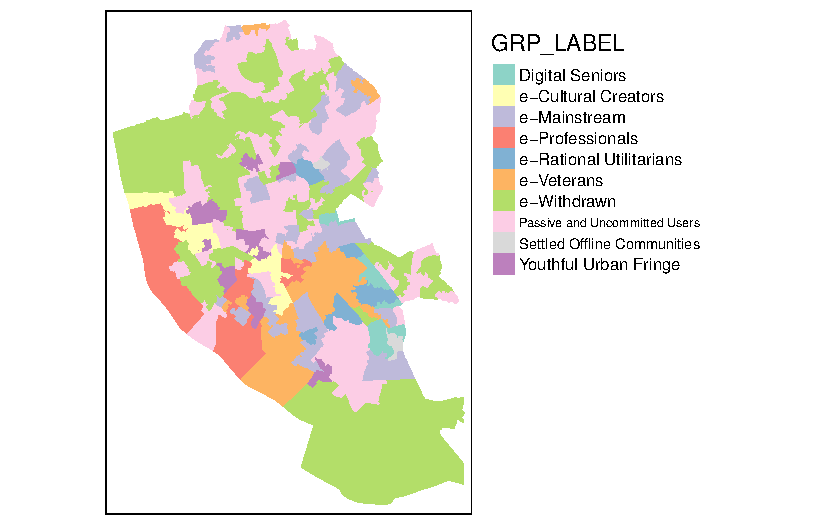
\includegraphics{01-geodemographics_files/figure-pdf/fig-geo-plot-those-spatial-data-1.pdf}

}

\caption{\label{fig-geo-plot-those-spatial-data}Internet User
Classification Liverpool}

\end{figure}

Let's use the same colours as used on
\href{https://mapmaker.cdrc.ac.uk/\#/internet-user-classification?lon=-2.81187\&lat=53.31045\&zoom=9.58}{CDRC
mapmaker} by specifying the \textbf{hex} colour codes for each of our
groups. Note the order of the colours is important: the colour for group
1 is first, group 2 second and so on.

\begin{codelisting}

\caption{\texttt{R code}}

\begin{Shaded}
\begin{Highlighting}[]
\CommentTok{\# define palette}
\NormalTok{iuc\_colours }\OtherTok{\textless{}{-}} \FunctionTok{c}\NormalTok{(}\StringTok{"\#dd7cdc"}\NormalTok{, }\StringTok{"\#ea4d78"}\NormalTok{, }\StringTok{"\#d2d1ab"}\NormalTok{, }\StringTok{"\#f36d5a"}\NormalTok{, }\StringTok{"\#a5cfbc"}\NormalTok{, }\StringTok{"\#e4a5d0"}\NormalTok{,}
    \StringTok{"\#8470ff"}\NormalTok{, }\StringTok{"\#79cdcd"}\NormalTok{, }\StringTok{"\#808fee"}\NormalTok{, }\StringTok{"\#ffd39b"}\NormalTok{)}

\CommentTok{\# plot pretty}
\FunctionTok{tm\_shape}\NormalTok{(liv\_iuc) }\SpecialCharTok{+} \FunctionTok{tm\_fill}\NormalTok{(}\AttributeTok{col =} \StringTok{"GRP\_LABEL"}\NormalTok{, }\AttributeTok{palette =}\NormalTok{ iuc\_colours) }\SpecialCharTok{+} \FunctionTok{tm\_layout}\NormalTok{(}\AttributeTok{legend.outside =} \ConstantTok{TRUE}\NormalTok{)}
\end{Highlighting}
\end{Shaded}

\end{codelisting}

\begin{figure}[H]

{\centering 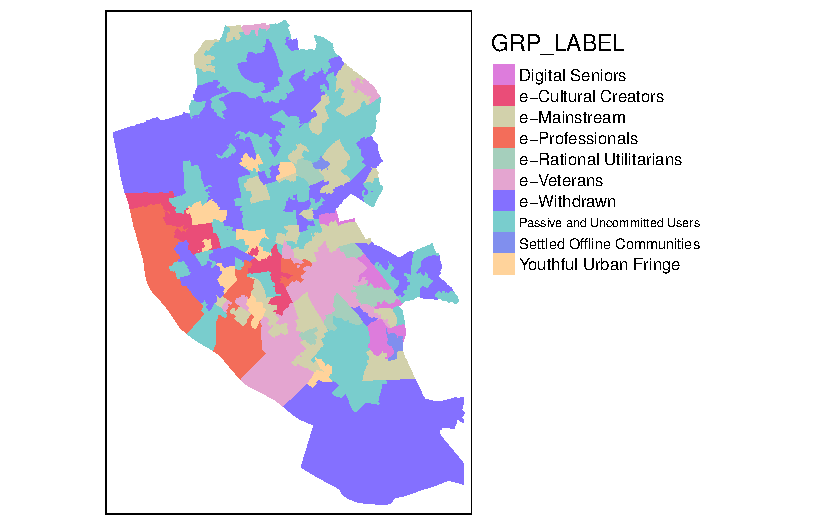
\includegraphics{01-geodemographics_files/figure-pdf/fig-geo-pretty-colours-1.pdf}

}

\caption{\label{fig-geo-pretty-colours}Internet User Classification
Liverpool with mapmaker colours}

\end{figure}

\hypertarget{task-geo-1}{%
\subsection{Tutorial task I}\label{task-geo-1}}

Now we have these cluster classifications, how can we link them to
people? Try using the \textbf{Mid-Year Population Estimates 2019} that
you can download below to:

\begin{itemize}
\tightlist
\item
  calculate the total number of people associated with each cluster
  group \textbf{for England and Wales as a whole}; and
\item
  create a pretty data visualisation showing the results (no map!).
\end{itemize}

\hypertarget{file-download}{%
\subsubsection*{File download}\label{file-download}}
\addcontentsline{toc}{subsubsection}{File download}

\begin{longtable}[]{@{}
  >{\raggedright\arraybackslash}p{(\columnwidth - 4\tabcolsep) * \real{0.5493}}
  >{\raggedright\arraybackslash}p{(\columnwidth - 4\tabcolsep) * \real{0.2254}}
  >{\raggedright\arraybackslash}p{(\columnwidth - 4\tabcolsep) * \real{0.2254}}@{}}
\toprule\noalign{}
\begin{minipage}[b]{\linewidth}\raggedright
File
\end{minipage} & \begin{minipage}[b]{\linewidth}\raggedright
Type
\end{minipage} & \begin{minipage}[b]{\linewidth}\raggedright
Link
\end{minipage} \\
\midrule\noalign{}
\endhead
\bottomrule\noalign{}
\endlastfoot
LSOA-level Mid-Year Population Estimates England and Wales 2019 &
\texttt{csv} &
\href{https://github.com/jtvandijk/GEOG0114/tree/master/data/zip/mye_pop_2019_lsoa.zip}{Download} \\
Lower-layer Super Output Areas Great Britain 2011 & \texttt{shp} &
\href{https://github.com/jtvandijk/GEOG0114/tree/master/data/zip/gb_lsoa11_sim.zip}{Download} \\
\end{longtable}

\hypertarget{k-means-clustering}{%
\subsection{k-means clustering}\label{k-means-clustering}}

In several cases, including the
\href{http://josis.org/index.php/josis/article/view/232/150}{2011
residential-based area classifications} and the Internet User
Classification, a technique called \textbf{k-means clustering} is used
in the creation of a geodemographic classification. K-means clustering
aims to partition a set of observations into a number of clusters
(\emph{k}), in which each observation will be assigned to the cluster
with the nearest mean. As such, a cluster refers to a collection of data
points aggregated together because of certain similarities
(i.e.~standardised scores of your input data). In order to run a
\textbf{k-means clustering}, you first define a target number \emph{k}
of clusters that you want. The k-means algorithm subsequently assigns
every observation to one of the clusters by finding the solution that
minimises the total within-cluster variance. For the second part of this
week's practical material, we will be replicating part of the Internet
User Classification for Great Britain. For this we will be using an
MSOA-level input data set containing various socio-demographic and
socio-economic variables that you can download below together with the
MSOA administrative boundaries.

The data set contains the following variables:

\begin{longtable}[]{@{}
  >{\raggedright\arraybackslash}p{(\columnwidth - 2\tabcolsep) * \real{0.5000}}
  >{\raggedright\arraybackslash}p{(\columnwidth - 2\tabcolsep) * \real{0.5000}}@{}}
\toprule\noalign{}
\begin{minipage}[b]{\linewidth}\raggedright
Variable
\end{minipage} & \begin{minipage}[b]{\linewidth}\raggedright
Definition
\end{minipage} \\
\midrule\noalign{}
\endhead
\bottomrule\noalign{}
\endlastfoot
\texttt{msoa11cd} & MSOA Code \\
\texttt{age\_total}, \texttt{age0to4pc}, \texttt{age5to14pc},
\texttt{age16to24pc}, \texttt{age25to44pc}, \texttt{age45to64pc},
\texttt{age75pluspc} & Percentage of people in various age groups \\
\texttt{nssec\_total}, \texttt{1\_higher\_managerial},
\texttt{2\_lower\_managerial}, \texttt{3\_intermediate\_occupations},
\texttt{4\_employers\_small\_org}, \texttt{5\_lower\_supervisory},
\texttt{6\_semi\_routine}, \texttt{7\_routine}, \texttt{8\_unemployed} &
Percentage of people in selected operational categories and
sub-categories classes drawn from the National Statistics Socio-economic
Classification
(\href{https://www.ons.gov.uk/methodology/classificationsandstandards/otherclassifications/thenationalstatisticssocioeconomicclassificationnssecrebasedonsoc2010}{NS-SEC}) \\
\texttt{avg\_dwn\_speed}, \texttt{avb\_superfast},
\texttt{no\_decent\_bband}, \texttt{bband\_speed\_under2mbs},
\texttt{bband\_speed\_under10mbs}, \texttt{bband\_speed\_over30mbs} &
Measures of broadband use and internet availability \\
\end{longtable}

\hypertarget{file-download-1}{%
\subsubsection*{File download}\label{file-download-1}}
\addcontentsline{toc}{subsubsection}{File download}

\begin{longtable}[]{@{}
  >{\raggedright\arraybackslash}p{(\columnwidth - 4\tabcolsep) * \real{0.5493}}
  >{\raggedright\arraybackslash}p{(\columnwidth - 4\tabcolsep) * \real{0.2254}}
  >{\raggedright\arraybackslash}p{(\columnwidth - 4\tabcolsep) * \real{0.2254}}@{}}
\toprule\noalign{}
\begin{minipage}[b]{\linewidth}\raggedright
File
\end{minipage} & \begin{minipage}[b]{\linewidth}\raggedright
Type
\end{minipage} & \begin{minipage}[b]{\linewidth}\raggedright
Link
\end{minipage} \\
\midrule\noalign{}
\endhead
\bottomrule\noalign{}
\endlastfoot
Middle-layer Super Output Areas Great Britain 2011 & \texttt{shp} &
\href{https://github.com/jtvandijk/GEOG0114/tree/master/data/zip/gb_msoa11_sim.zip}{Download} \\
MSOA-level input variables for IUC & \texttt{csv} &
\href{https://github.com/jtvandijk/GEOG0114/tree/master/data/zip/msoa_iuc_input.zip}{Download} \\
\end{longtable}

\begin{codelisting}

\caption{\texttt{R code}}

\begin{Shaded}
\begin{Highlighting}[]
\CommentTok{\# load data}
\NormalTok{iuc\_input }\OtherTok{\textless{}{-}} \FunctionTok{read\_csv}\NormalTok{(}\StringTok{"data/index/msoa{-}iuc{-}input.csv"}\NormalTok{)}

\CommentTok{\# inspect}
\FunctionTok{head}\NormalTok{(iuc\_input)}
\end{Highlighting}
\end{Shaded}

\end{codelisting}

\begin{verbatim}
# A tibble: 6 x 23
  msoa11cd  age_total age0to4pc age5to~1 age16~2 age25~3 age45~4 age75~5 nssec~6
  <chr>         <dbl>     <dbl>    <dbl>   <dbl>   <dbl>   <dbl>   <dbl>   <dbl>
1 E02000001      7375    0.032    0.0388  0.0961   0.407   0.273  0.0607    5816
2 E02000002      6775    0.0927   0.122   0.113    0.280   0.186  0.0980    3926
3 E02000003     10045    0.0829   0.102   0.118    0.306   0.225  0.0646    6483
4 E02000004      6182    0.0590   0.102   0.139    0.254   0.250  0.0886    4041
5 E02000005      8562    0.0930   0.119   0.119    0.299   0.214  0.0501    5368
6 E02000007      8791    0.103    0.125   0.129    0.285   0.197  0.0688    5158
# ... with 14 more variables: `1_higher_managerial` <dbl>,
#   `2_lower_managerial` <dbl>, `3_intermediate_occupations` <dbl>,
#   `4_employers_small_org` <dbl>, `5_lower_supervisory` <dbl>,
#   `6_semi_routine` <dbl>, `7_routine` <dbl>, `8_unemployed` <dbl>,
#   avg_dwn_speed <dbl>, avb_superfast <dbl>, no_decent_bband <dbl>,
#   bband_speed_under2mbs <dbl>, bband_speed_under10mbs <dbl>,
#   bband_speed_over30mbs <dbl>, and abbreviated variable names ...
\end{verbatim}

Before running our \textbf{k-means} clustering algorithm, we need to
extract the data which we want to use; i.e.~we need to remove all the
columns with data that we do not want to include in the clustering
process.

\begin{codelisting}

\caption{\texttt{R code}}

\begin{Shaded}
\begin{Highlighting}[]
\CommentTok{\# column names}
\FunctionTok{names}\NormalTok{(iuc\_input)}
\end{Highlighting}
\end{Shaded}

\end{codelisting}

\begin{verbatim}
 [1] "msoa11cd"                   "age_total"                 
 [3] "age0to4pc"                  "age5to14pc"                
 [5] "age16to24pc"                "age25to44pc"               
 [7] "age45to64pc"                "age75pluspc"               
 [9] "nssec_total"                "1_higher_managerial"       
[11] "2_lower_managerial"         "3_intermediate_occupations"
[13] "4_employers_small_org"      "5_lower_supervisory"       
[15] "6_semi_routine"             "7_routine"                 
[17] "8_unemployed"               "avg_dwn_speed"             
[19] "avb_superfast"              "no_decent_bband"           
[21] "bband_speed_under2mbs"      "bband_speed_under10mbs"    
[23] "bband_speed_over30mbs"     
\end{verbatim}

\begin{Shaded}
\begin{Highlighting}[]
\CommentTok{\# extract columns by index}
\NormalTok{cluster\_data }\OtherTok{\textless{}{-}}\NormalTok{ iuc\_input[, }\FunctionTok{c}\NormalTok{(}\DecValTok{3}\SpecialCharTok{:}\DecValTok{8}\NormalTok{, }\DecValTok{10}\SpecialCharTok{:}\DecValTok{17}\NormalTok{, }\DecValTok{18}\SpecialCharTok{:}\DecValTok{20}\NormalTok{)]}

\CommentTok{\# inspect}
\FunctionTok{head}\NormalTok{(cluster\_data)}
\end{Highlighting}
\end{Shaded}

\begin{verbatim}
# A tibble: 6 x 17
  age0to4pc age5to14pc age16to~1 age25~2 age45~3 age75~4 1_hig~5 2_low~6 3_int~7
      <dbl>      <dbl>     <dbl>   <dbl>   <dbl>   <dbl>   <dbl>   <dbl>   <dbl>
1    0.032      0.0388    0.0961   0.407   0.273  0.0607  0.385    0.339  0.0781
2    0.0927     0.122     0.113    0.280   0.186  0.0980  0.0568   0.171  0.143 
3    0.0829     0.102     0.118    0.306   0.225  0.0646  0.0818   0.208  0.182 
4    0.0590     0.102     0.139    0.254   0.250  0.0886  0.0678   0.206  0.191 
5    0.0930     0.119     0.119    0.299   0.214  0.0501  0.0494   0.166  0.156 
6    0.103      0.125     0.129    0.285   0.197  0.0688  0.0564   0.163  0.136 
# ... with 8 more variables: `4_employers_small_org` <dbl>,
#   `5_lower_supervisory` <dbl>, `6_semi_routine` <dbl>, `7_routine` <dbl>,
#   `8_unemployed` <dbl>, avg_dwn_speed <dbl>, avb_superfast <dbl>,
#   no_decent_bband <dbl>, and abbreviated variable names 1: age16to24pc,
#   2: age25to44pc, 3: age45to64pc, 4: age75pluspc, 5: `1_higher_managerial`,
#   6: `2_lower_managerial`, 7: `3_intermediate_occupations`
\end{verbatim}

We also need to rescale the data so all input data are presented on a
comparable scale: the average download speed data
(i.e.~\texttt{avg\_dwn\_speed}) is very different to the other data
that, for instance, represent the percentage of the population by
different age groups.

\begin{codelisting}

\caption{\texttt{R code}}

\begin{Shaded}
\begin{Highlighting}[]
\CommentTok{\# rescale}
\NormalTok{cluster\_data }\OtherTok{\textless{}{-}} \FunctionTok{scale}\NormalTok{(cluster\_data)}

\CommentTok{\# inspect}
\FunctionTok{head}\NormalTok{(cluster\_data)}
\end{Highlighting}
\end{Shaded}

\end{codelisting}

\begin{verbatim}
      age0to4pc age5to14pc age16to24pc age25to44pc age45to64pc age75pluspc
[1,] -1.7579913 -2.8680309 -0.36823669   2.1768529   0.2561260  -0.6039803
[2,]  1.9519376  1.6403191 -0.05766949   0.1671857  -1.5639740   0.6215590
[3,]  1.3549320  0.5475394  0.02888699   0.5773908  -0.7424464  -0.4769094
[4,] -0.1050147  0.5938501  0.40759191  -0.2402277  -0.2247116   0.3136111
[5,]  1.9687596  1.5173858  0.05639359   0.4733916  -0.9785969  -0.9539525
[6,]  2.6064366  1.8434062  0.22116720   0.2379171  -1.3168781  -0.3384050
     1_higher_managerial 2_lower_managerial 3_intermediate_occupations
[1,]           4.4185012          1.8391416                 -2.2291104
[2,]          -0.8510113         -0.9272602                  0.1031344
[3,]          -0.4499409         -0.3266302                  1.5123844
[4,]          -0.6741298         -0.3469851                  1.8104058
[5,]          -0.9705088         -1.0065195                  0.5809449
[6,]          -0.8571773         -1.0674213                 -0.1494470
     4_employers_small_org 5_lower_supervisory 6_semi_routine   7_routine
[1,]           -1.02298662         -2.53130431    -2.49888739 -1.81145433
[2,]            0.39745656         -0.67859270     1.05051667  0.08877827
[3,]            0.28308676         -0.37987493    -0.05595897 -0.52802287
[4,]            0.13591535          0.24587683    -0.15093353 -0.07008362
[5,]            0.09942212          0.42532220     0.76747039  0.35318453
[6,]           -0.18786941          0.05518013     0.56442659  0.57156979
     8_unemployed avg_dwn_speed avb_superfast no_decent_bband
[1,]   -0.5139854    -1.6561653    -5.2186970      -0.3797659
[2,]    1.1777334     0.7915882     0.5093876      -0.2031415
[3,]    0.7615830     0.6354463     0.5222597      -0.3797659
[4,]    0.2898589     0.9477301     0.5480039      -0.2472976
[5,]    0.8482656     0.4701196     0.2648177       0.2384195
[6,]    1.5510655     0.6813704     0.4965155      -0.1589854
\end{verbatim}

Now our data are all on the same scale, we will start by creating an
elbow plot. The
\href{https://en.wikipedia.org/wiki/Elbow_method_(clustering)\#:~:text=In\%20cluster\%20analysis\%2C\%20the\%20elbow,number\%20of\%20clusters\%20to\%20use\%60}{elbow
method} is a visual aid that can help in determining the number of
clusters in a data set. Remember: this is important because with a
\textbf{k-means} clustering you need to specify the numbers of clusters
\emph{a priori}!

The elbow method can help as it plots the total explained variation
(`Within Sum of Squares') in your data as a function of the number of
cluster. The idea is that you pick the number of clusters at the `elbow'
of the curve as this is the point in which the additional variation that
would be explained by an additional cluster is decreasing. Effectively
this means you are actually running the \textbf{k-means} clustering
multiple times before running the actual \textbf{k-means} clustering
algorithm.

\begin{codelisting}

\caption{\texttt{R code}}

\begin{Shaded}
\begin{Highlighting}[]
\CommentTok{\# create empty list to store the within sum of square values}
\NormalTok{wss\_values }\OtherTok{\textless{}{-}} \FunctionTok{list}\NormalTok{()}

\CommentTok{\# execute a k{-}means clustering for k=1, k=2, ..., k=15}
\ControlFlowTok{for}\NormalTok{ (i }\ControlFlowTok{in} \DecValTok{1}\SpecialCharTok{:}\DecValTok{15}\NormalTok{) \{}
\NormalTok{    wss\_values[i] }\OtherTok{\textless{}{-}} \FunctionTok{sum}\NormalTok{(}\FunctionTok{kmeans}\NormalTok{(cluster\_data, }\AttributeTok{centers =}\NormalTok{ i, }\AttributeTok{iter.max =} \DecValTok{30}\NormalTok{)}\SpecialCharTok{$}\NormalTok{withinss)}
\NormalTok{\}}

\CommentTok{\# inspect}
\NormalTok{wss\_values}
\end{Highlighting}
\end{Shaded}

\end{codelisting}

\begin{verbatim}
[[1]]
[1] 144143

[[2]]
[1] 110934.1

[[3]]
[1] 100058.1

[[4]]
[1] 82701.63

[[5]]
[1] 73974.97

 [ reached getOption("max.print") -- omitted 10 entries ]
\end{verbatim}

\begin{codelisting}

\caption{\texttt{R code}}

\begin{Shaded}
\begin{Highlighting}[]
\CommentTok{\# vector to dataframe}
\NormalTok{wss\_values }\OtherTok{\textless{}{-}} \FunctionTok{as.data.frame}\NormalTok{(wss\_values)}

\CommentTok{\# transpose}
\NormalTok{wss\_values }\OtherTok{\textless{}{-}} \FunctionTok{as.data.frame}\NormalTok{(}\FunctionTok{t}\NormalTok{(wss\_values))}

\CommentTok{\# add cluster numbers}
\NormalTok{wss\_values}\SpecialCharTok{$}\NormalTok{cluster }\OtherTok{\textless{}{-}} \FunctionTok{seq.int}\NormalTok{(}\FunctionTok{nrow}\NormalTok{(wss\_values))}
\FunctionTok{names}\NormalTok{(wss\_values) }\OtherTok{\textless{}{-}} \FunctionTok{c}\NormalTok{(}\StringTok{"wss"}\NormalTok{, }\StringTok{"cluster"}\NormalTok{)}

\CommentTok{\# plot using ggplot2}
\FunctionTok{ggplot}\NormalTok{(}\AttributeTok{data =}\NormalTok{ wss\_values, }\FunctionTok{aes}\NormalTok{(}\AttributeTok{x =}\NormalTok{ cluster, }\AttributeTok{y =}\NormalTok{ wss)) }\SpecialCharTok{+} \FunctionTok{geom\_point}\NormalTok{() }\SpecialCharTok{+} \FunctionTok{geom\_path}\NormalTok{() }\SpecialCharTok{+}
    \FunctionTok{scale\_x\_continuous}\NormalTok{(}\AttributeTok{breaks =} \FunctionTok{seq}\NormalTok{(}\DecValTok{1}\NormalTok{, }\DecValTok{15}\NormalTok{)) }\SpecialCharTok{+} \FunctionTok{xlab}\NormalTok{(}\StringTok{"Number of clusters"}\NormalTok{) }\SpecialCharTok{+} \FunctionTok{ylab}\NormalTok{(}\StringTok{"Within sum of squares"}\NormalTok{) }\SpecialCharTok{+}
    \FunctionTok{theme\_minimal}\NormalTok{()}
\end{Highlighting}
\end{Shaded}

\end{codelisting}

\begin{figure}[H]

{\centering 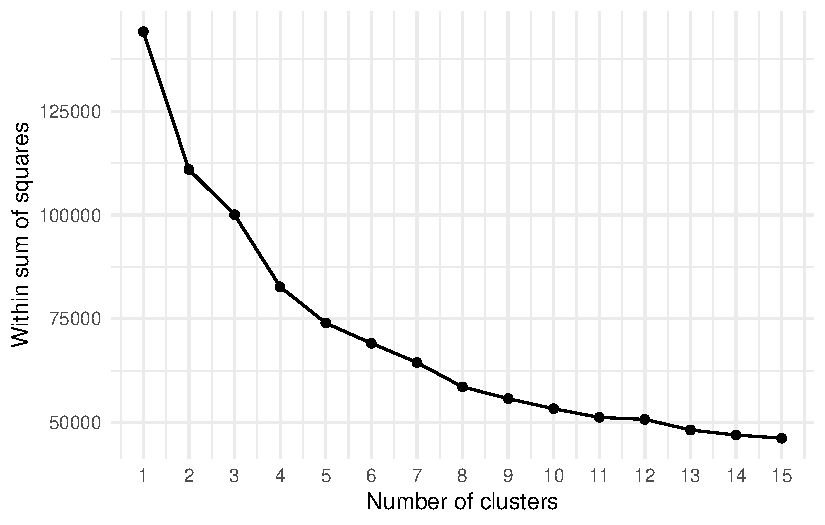
\includegraphics{01-geodemographics_files/figure-pdf/fig-geo-variables-that-cluster-1.pdf}

}

\caption{\label{fig-geo-variables-that-cluster}Within sum of squares by
number of clusters}

\end{figure}

Based on the elbow plot, we can now choose the number of clusters and it
looks like \textbf{7} clusters would be a reasonable choice.

\begin{tcolorbox}[enhanced jigsaw, rightrule=.15mm, colback=white, opacityback=0, opacitybacktitle=0.6, coltitle=black, colbacktitle=quarto-callout-note-color!10!white, breakable, arc=.35mm, title=\textcolor{quarto-callout-note-color}{\faInfo}\hspace{0.5em}{Note}, left=2mm, leftrule=.75mm, bottomtitle=1mm, toprule=.15mm, bottomrule=.15mm, colframe=quarto-callout-note-color-frame, toptitle=1mm, titlerule=0mm]

The interpretation of an elbow plot can be quite subjective and often
multiple options would be justified: \textbf{6}, \textbf{8}, and perhaps
\textbf{9} clusters also do not look unreasonable. You would need to try
the different options and see what output you get to determine the
`optimal' solution. However, at very least, the elbow plot does give you
an idea of what would potentially be an adequate number of clusters.

\end{tcolorbox}

Now we have decided on the number of clusters (i.e.~\textbf{7}
clusters), we can run our cluster analysis. We will be running this
analysis 10 times because there is an element of randomness within the
clustering, and we want to make sure we get the optimal clustering
output.

\begin{codelisting}

\caption{\texttt{R code}}

\begin{Shaded}
\begin{Highlighting}[]
\CommentTok{\# create empty list to store the results of the clustering}
\NormalTok{clusters }\OtherTok{\textless{}{-}} \FunctionTok{list}\NormalTok{()}

\CommentTok{\# create empty variable to store fit}
\NormalTok{fit }\OtherTok{\textless{}{-}} \ConstantTok{NA}

\CommentTok{\# run the k{-}means 10 times}
\ControlFlowTok{for}\NormalTok{ (i }\ControlFlowTok{in} \DecValTok{1}\SpecialCharTok{:}\DecValTok{10}\NormalTok{) \{}

    \CommentTok{\# keep track of the runs}
    \FunctionTok{print}\NormalTok{(}\FunctionTok{paste0}\NormalTok{(}\StringTok{"starting run: "}\NormalTok{, i))}

    \CommentTok{\# run the k{-}means clustering algorithm to extract 7 clusters}
\NormalTok{    clust7 }\OtherTok{\textless{}{-}} \FunctionTok{kmeans}\NormalTok{(}\AttributeTok{x =}\NormalTok{ cluster\_data, }\AttributeTok{centers =} \DecValTok{7}\NormalTok{, }\AttributeTok{iter.max =} \FloatTok{1e+06}\NormalTok{, }\AttributeTok{nstart =} \DecValTok{1}\NormalTok{)}

    \CommentTok{\# get the total within sum of squares for the run and}
\NormalTok{    fit[i] }\OtherTok{\textless{}{-}}\NormalTok{ clust7}\SpecialCharTok{$}\NormalTok{tot.withinss}

    \CommentTok{\# update the results of the clustering if the total within sum of squares}
    \CommentTok{\# for the run is lower than any of the runs that have been executed so far}
    \ControlFlowTok{if}\NormalTok{ (fit[i] }\SpecialCharTok{\textless{}} \FunctionTok{min}\NormalTok{(fit[}\DecValTok{1}\SpecialCharTok{:}\NormalTok{(i }\SpecialCharTok{{-}} \DecValTok{1}\NormalTok{)])) \{}
\NormalTok{        clusters }\OtherTok{\textless{}{-}}\NormalTok{ clust7}
\NormalTok{    \}}
\NormalTok{\}}
\end{Highlighting}
\end{Shaded}

\end{codelisting}

\begin{verbatim}
[1] "starting run: 1"
[1] "starting run: 2"
[1] "starting run: 3"
[1] "starting run: 4"
[1] "starting run: 5"
[1] "starting run: 6"
[1] "starting run: 7"
[1] "starting run: 8"
[1] "starting run: 9"
[1] "starting run: 10"
\end{verbatim}

\begin{Shaded}
\begin{Highlighting}[]
\CommentTok{\# inspect}
\NormalTok{clusters}
\end{Highlighting}
\end{Shaded}

\begin{verbatim}
K-means clustering with 7 clusters of sizes 2053, 2039, 740, 186, 1107, 1814, 541

Cluster means:
     age0to4pc  age5to14pc age16to24pc age25to44pc age45to64pc age75pluspc
  1_higher_managerial 2_lower_managerial 3_intermediate_occupations
  4_employers_small_org 5_lower_supervisory 6_semi_routine  7_routine
  8_unemployed avg_dwn_speed avb_superfast no_decent_bband
 [ reached getOption("max.print") -- omitted 7 rows ]

Clustering vector:
[1] 3 5 2 2 5
 [ reached getOption("max.print") -- omitted 8475 entries ]

Within cluster sum of squares by cluster:
[1] 11736.830 11471.872  7786.692  3401.821  9429.647
 [ reached getOption("max.print") -- omitted 2 entries ]
 (between_SS / total_SS =  56.3 %)

Available components:

[1] "cluster"      "centers"      "totss"        "withinss"     "tot.withinss"
 [ reached getOption("max.print") -- omitted 4 entries ]
\end{verbatim}

We now have to execute a bit of post-processing to extract some useful
summary data for each cluster: the cluster size (\texttt{size}) and mean
values for each cluster.

\begin{codelisting}

\caption{\texttt{R code}}

\begin{Shaded}
\begin{Highlighting}[]
\CommentTok{\# assign to new variable for clarity}
\NormalTok{kfit }\OtherTok{\textless{}{-}}\NormalTok{ clusters}

\CommentTok{\# cluster sizes}
\NormalTok{kfit\_size }\OtherTok{\textless{}{-}}\NormalTok{ kfit}\SpecialCharTok{$}\NormalTok{size}

\CommentTok{\# inspect}
\NormalTok{kfit\_size}
\end{Highlighting}
\end{Shaded}

\end{codelisting}

\begin{verbatim}
[1] 2053 2039  740  186 1107
 [ reached getOption("max.print") -- omitted 2 entries ]
\end{verbatim}

\begin{Shaded}
\begin{Highlighting}[]
\CommentTok{\# mean values for each variable in each cluster}
\NormalTok{kfit\_mean }\OtherTok{\textless{}{-}} \FunctionTok{as\_tibble}\NormalTok{(}\FunctionTok{aggregate}\NormalTok{(cluster\_data, }\AttributeTok{by =} \FunctionTok{list}\NormalTok{(kfit}\SpecialCharTok{$}\NormalTok{cluster), }\AttributeTok{FUN =}\NormalTok{ mean))}
\FunctionTok{names}\NormalTok{(kfit\_mean)[}\DecValTok{1}\NormalTok{] }\OtherTok{\textless{}{-}} \StringTok{"cluster"}

\CommentTok{\# inspect}
\NormalTok{kfit\_mean}
\end{Highlighting}
\end{Shaded}

\begin{verbatim}
# A tibble: 7 x 18
  cluster age0to4pc age5to14pc age16to~1 age25~2 age45~3 age75~4 1_hig~5 2_low~6
    <int>     <dbl>      <dbl>     <dbl>   <dbl>   <dbl>   <dbl>   <dbl>   <dbl>
1       1  -0.00815    -0.0824   -0.0526 -0.158   0.0919   0.164 -0.837   -0.849
2       2   0.0162      0.118    -0.172   0.0189  0.202   -0.103 -0.0481   0.211
3       3   0.326      -0.923     0.209   2.05   -1.23    -0.927  1.50     1.26 
4       4  -1.52       -2.68      5.42    0.113  -2.62    -1.28   0.870    0.223
5       5   1.56        1.14      0.381   0.626  -1.13    -0.954 -0.906   -1.26 
6       6  -0.679      -0.0412   -0.465  -0.773   0.765    0.856  0.845    0.893
7       7  -0.880      -0.148    -0.523  -0.998   1.22     0.554  0.0251   0.225
# ... with 9 more variables: `3_intermediate_occupations` <dbl>,
#   `4_employers_small_org` <dbl>, `5_lower_supervisory` <dbl>,
#   `6_semi_routine` <dbl>, `7_routine` <dbl>, `8_unemployed` <dbl>,
#   avg_dwn_speed <dbl>, avb_superfast <dbl>, no_decent_bband <dbl>, and
#   abbreviated variable names 1: age16to24pc, 2: age25to44pc, 3: age45to64pc,
#   4: age75pluspc, 5: `1_higher_managerial`, 6: `2_lower_managerial`
\end{verbatim}

\begin{codelisting}

\caption{\texttt{R code}}

\begin{Shaded}
\begin{Highlighting}[]
\CommentTok{\# transform shape to tidy format}
\NormalTok{kfit\_mean\_long }\OtherTok{\textless{}{-}} \FunctionTok{pivot\_longer}\NormalTok{(kfit\_mean, }\AttributeTok{cols =}\NormalTok{ (}\SpecialCharTok{{-}}\NormalTok{cluster))}

\CommentTok{\# plot using ggplot2}
\FunctionTok{ggplot}\NormalTok{(kfit\_mean\_long, }\FunctionTok{aes}\NormalTok{(}\AttributeTok{x =}\NormalTok{ cluster, }\AttributeTok{y =}\NormalTok{ value, }\AttributeTok{fill =}\NormalTok{ name)) }\SpecialCharTok{+} \FunctionTok{geom\_bar}\NormalTok{(}\AttributeTok{stat =} \StringTok{"identity"}\NormalTok{,}
    \AttributeTok{position =} \StringTok{"dodge"}\NormalTok{) }\SpecialCharTok{+} \FunctionTok{scale\_x\_continuous}\NormalTok{(}\AttributeTok{breaks =} \FunctionTok{seq}\NormalTok{(}\DecValTok{1}\NormalTok{, }\DecValTok{7}\NormalTok{, }\AttributeTok{by =} \DecValTok{1}\NormalTok{)) }\SpecialCharTok{+} \FunctionTok{xlab}\NormalTok{(}\StringTok{"Cluster"}\NormalTok{) }\SpecialCharTok{+}
    \FunctionTok{ylab}\NormalTok{(}\StringTok{"Mean value"}\NormalTok{) }\SpecialCharTok{+} \FunctionTok{theme\_minimal}\NormalTok{() }\SpecialCharTok{+} \FunctionTok{theme}\NormalTok{(}\AttributeTok{legend.title =} \FunctionTok{element\_blank}\NormalTok{(),}
    \AttributeTok{legend.position =} \StringTok{"bottom"}\NormalTok{)}
\end{Highlighting}
\end{Shaded}

\end{codelisting}

\begin{figure}[H]

{\centering 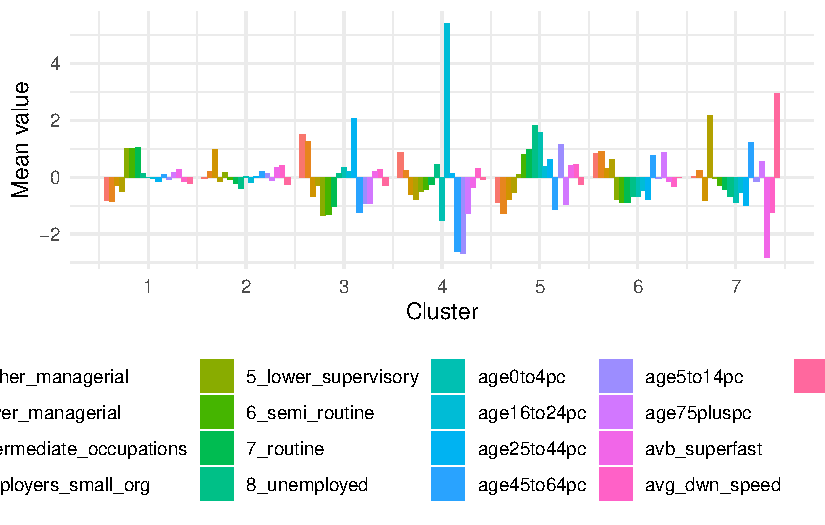
\includegraphics{01-geodemographics_files/figure-pdf/fig-geo-plot-those-clusters-with-a-graph-1.pdf}

}

\caption{\label{fig-geo-plot-those-clusters-with-a-graph}Mean variable
values by cluster}

\end{figure}

\begin{tcolorbox}[enhanced jigsaw, rightrule=.15mm, colback=white, opacityback=0, opacitybacktitle=0.6, coltitle=black, colbacktitle=quarto-callout-warning-color!10!white, breakable, arc=.35mm, title=\textcolor{quarto-callout-warning-color}{\faExclamationTriangle}\hspace{0.5em}{Warning}, left=2mm, leftrule=.75mm, bottomtitle=1mm, toprule=.15mm, bottomrule=.15mm, colframe=quarto-callout-warning-color-frame, toptitle=1mm, titlerule=0mm]

Your values may be slightly different due to the random choice of
initial cluster centres.

\end{tcolorbox}

Looking at the table with the mean values for each cluster and the
barplot, we can see that variables contribute differently to the
different clusters. The graph is a little busy, so you might want to
look at the cluster groups or variables individually to get a better
picture of each cluster.

\begin{codelisting}

\caption{\texttt{R code}}

\begin{Shaded}
\begin{Highlighting}[]
\CommentTok{\# plot using ggplot2}
\FunctionTok{ggplot}\NormalTok{(kfit\_mean\_long[kfit\_mean\_long}\SpecialCharTok{$}\NormalTok{cluster }\SpecialCharTok{==} \DecValTok{1}\NormalTok{, ], }\FunctionTok{aes}\NormalTok{(}\AttributeTok{x =}\NormalTok{ cluster, }\AttributeTok{y =}\NormalTok{ value,}
    \AttributeTok{fill =}\NormalTok{ name)) }\SpecialCharTok{+} \FunctionTok{geom\_bar}\NormalTok{(}\AttributeTok{stat =} \StringTok{"identity"}\NormalTok{, }\AttributeTok{position =} \StringTok{"dodge"}\NormalTok{) }\SpecialCharTok{+} \FunctionTok{xlab}\NormalTok{(}\StringTok{"Cluster"}\NormalTok{) }\SpecialCharTok{+}
    \FunctionTok{ylab}\NormalTok{(}\StringTok{"Mean value"}\NormalTok{) }\SpecialCharTok{+} \FunctionTok{theme\_minimal}\NormalTok{() }\SpecialCharTok{+} \FunctionTok{theme}\NormalTok{(}\AttributeTok{legend.title =} \FunctionTok{element\_blank}\NormalTok{(),}
    \AttributeTok{legend.position =} \StringTok{"bottom"}\NormalTok{)}
\end{Highlighting}
\end{Shaded}

\end{codelisting}

\begin{figure}[H]

{\centering 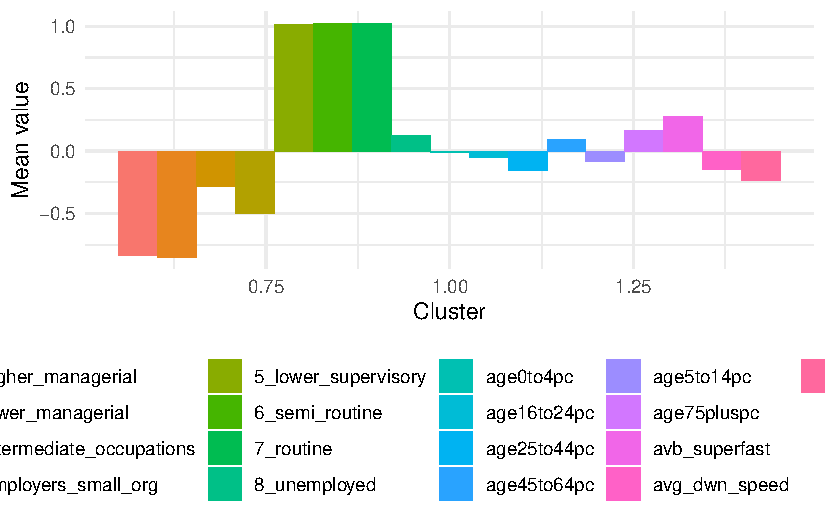
\includegraphics{01-geodemographics_files/figure-pdf/fig-geo-plot-those-clusters-with-a-graph-just-one-1.pdf}

}

\caption{\label{fig-geo-plot-those-clusters-with-a-graph-just-one}Mean
variable values for cluster 1}

\end{figure}

We can also show the results of our geodemographic classification on a
map.

\begin{codelisting}

\caption{\texttt{R code}}

\begin{Shaded}
\begin{Highlighting}[]
\CommentTok{\# read shape}
\NormalTok{msoa }\OtherTok{\textless{}{-}} \FunctionTok{st\_read}\NormalTok{(}\StringTok{"data/boundaries/gb\_msoa11\_sim.shp"}\NormalTok{)}
\end{Highlighting}
\end{Shaded}

\end{codelisting}

\begin{verbatim}
Reading layer `gb_msoa11_sim' from data source 
  `/Users/justinvandijk/Library/CloudStorage/Dropbox/UCL/Web/jtvandijk.github.io/GEOG0114Q/data/boundaries/gb_msoa11_sim.shp' 
  using driver `ESRI Shapefile'
Simple feature collection with 8480 features and 3 fields
Geometry type: MULTIPOLYGON
Dimension:     XY
Bounding box:  xmin: 5513 ymin: 5342.7 xmax: 655604.7 ymax: 1220302
Geodetic CRS:  WGS 84
\end{verbatim}

\begin{Shaded}
\begin{Highlighting}[]
\CommentTok{\# set projection}
\FunctionTok{st\_crs}\NormalTok{(msoa) }\OtherTok{=} \DecValTok{27700}

\CommentTok{\# simplify for speedier plotting}
\NormalTok{msoa }\OtherTok{\textless{}{-}} \FunctionTok{st\_simplify}\NormalTok{(msoa, }\AttributeTok{dTolerance =} \DecValTok{100}\NormalTok{)}

\CommentTok{\# join}
\NormalTok{cluster\_data }\OtherTok{\textless{}{-}} \FunctionTok{cbind}\NormalTok{(iuc\_input, kfit}\SpecialCharTok{$}\NormalTok{cluster)}
\NormalTok{msoa }\OtherTok{\textless{}{-}} \FunctionTok{left\_join}\NormalTok{(msoa, cluster\_data, }\AttributeTok{by =} \FunctionTok{c}\NormalTok{(}\AttributeTok{geo\_code =} \StringTok{"msoa11cd"}\NormalTok{))}

\CommentTok{\# plot}
\FunctionTok{tm\_shape}\NormalTok{(msoa) }\SpecialCharTok{+} \FunctionTok{tm\_fill}\NormalTok{(}\AttributeTok{col =} \StringTok{"kfit$cluster"}\NormalTok{) }\SpecialCharTok{+} \FunctionTok{tm\_layout}\NormalTok{(}\AttributeTok{legend.outside =} \ConstantTok{TRUE}\NormalTok{)}
\end{Highlighting}
\end{Shaded}

\begin{figure}[H]

{\centering 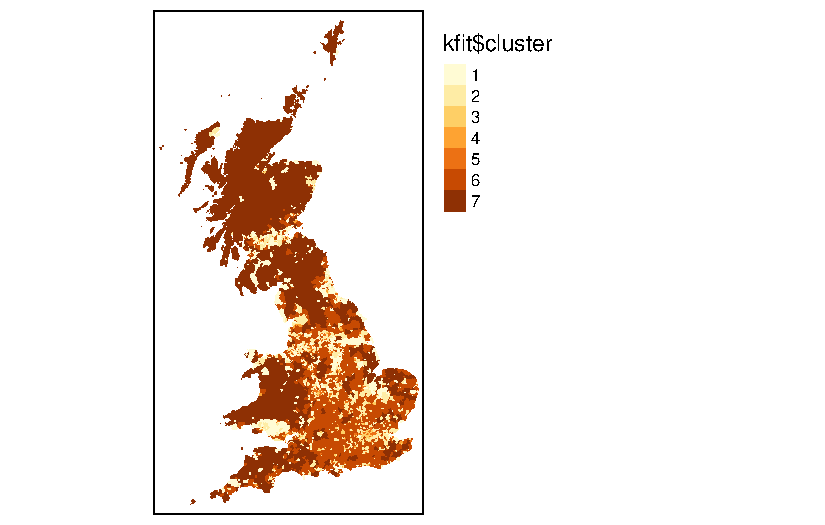
\includegraphics{01-geodemographics_files/figure-pdf/fig-geo-map-the-iuc-1.pdf}

}

\caption{\label{fig-geo-map-the-iuc}Spatial pattern of our
geodemographic classification}

\end{figure}

\begin{tcolorbox}[enhanced jigsaw, rightrule=.15mm, colback=white, opacityback=0, opacitybacktitle=0.6, coltitle=black, colbacktitle=quarto-callout-warning-color!10!white, breakable, arc=.35mm, title=\textcolor{quarto-callout-warning-color}{\faExclamationTriangle}\hspace{0.5em}{Warning}, left=2mm, leftrule=.75mm, bottomtitle=1mm, toprule=.15mm, bottomrule=.15mm, colframe=quarto-callout-warning-color-frame, toptitle=1mm, titlerule=0mm]

Your map might look different as the cluster numbers are not
consistently assigned and therefore colours can be map onto the cluster
numbers differently.

\end{tcolorbox}

\hypertarget{task-geo-2}{%
\subsection{Tutorial task II}\label{task-geo-2}}

The creation of a geodemographic classification is an \textbf{iterative
process} of trial and error that involves the addition and removal of
variables as well as experimentation with different numbers of clusters.
It also might be, for instances, that some clusters are very focused on
one group of data (e.g.~age) and it could be an idea to group some ages
together. If you want to make changes to the clustering solution, you
can simply re-run the analysis with a different set of variables or with
a different number of clusters by updating the code. However, it would
be even simpler if you could automate some of the process.

Try to create a \textbf{R function} that:

\begin{enumerate}
\def\labelenumi{\arabic{enumi}.}
\tightlist
\item
  takes \emph{at least} the following three arguments: \textbf{a data
  frame that contains your input data}, \textbf{the number of clusters
  that you want}, and \textbf{a list of input variables};
\item
  executes a \textbf{k-means} clustering on the input variables and the
  specified number of clusters; and,
\item
  produces a \texttt{csv} file that contains the \textbf{table of means}
  of the solution.
\end{enumerate}

\begin{tcolorbox}[enhanced jigsaw, rightrule=.15mm, colback=white, opacityback=0, opacitybacktitle=0.6, coltitle=black, colbacktitle=quarto-callout-note-color!10!white, breakable, arc=.35mm, title=\textcolor{quarto-callout-note-color}{\faInfo}\hspace{0.5em}{Note}, left=2mm, leftrule=.75mm, bottomtitle=1mm, toprule=.15mm, bottomrule=.15mm, colframe=quarto-callout-note-color-frame, toptitle=1mm, titlerule=0mm]

\begin{enumerate}
\def\labelenumi{\arabic{enumi}.}
\tightlist
\item
  Your function could look something like:
  \texttt{run-kmeans(dataframe,number\_of\_clusters,input\_variables)}
\item
  The list of input variables does not have to be a list of
  \emph{names}, but can also be a list containing the index values of
  the columns.
\item
  Have a look at \href{https://r4ds.had.co.nz/functions.html}{Hadley
  Wickhams explanation of functions} in R.
\end{enumerate}

\end{tcolorbox}

\hypertarget{byl-geo}{%
\section{Before you leave}\label{byl-geo}}

Having finished this tutorial, you should now understand the basics of a
geodemographic classification. In addition, you should have written a
simple function. Although
\href{https://www.youtube.com/watch?v=8iwBM_YB1sE}{you have now reached
the end of this week's content}, you could try and improve your
function. Consider:

\begin{enumerate}
\def\labelenumi{\arabic{enumi}.}
\tightlist
\item
  Including \emph{maps} or \emph{graphs} in the code that get
  automatically saved.
\item
  Ensuring that the \texttt{csv} outcome does \textbf{not} get
  overwritten every time you run you function.
\item
  Including optional arguments in your function with \textbf{default
  values} if certain values are not specified.
\end{enumerate}

\bookmarksetup{startatroot}

\hypertarget{transport-network-analysis}{%
\chapter{Transport Network Analysis}\label{transport-network-analysis}}

This week we will cover a different type of data: network data. We will
take a look at how we can use network data to measure accessibility
using the \texttt{dodgr} R library. We will calculate the network
distances between combinations of locations (i.e.~a set of origins and a
set of destinations). These distances can then, for instance, be used to
calculate the number of a resource (e.g.~fast-food outlets) within a
certain distance of a Point of Interest (e.g.~a school or
population-weighted centroid).

\hypertarget{lecture-w08}{%
\section{Lecture slides}\label{lecture-w08}}

You can download the slides of this week's lecture here:
\href{https://github.com/jtvandijk/GEOG0114Q/tree/master/slides/w08-psa.pdf}{{[}Link{]}}.

\hypertarget{reading-w08}{%
\section{Reading list}\label{reading-w08}}

\hypertarget{essential-readings-1}{%
\subsubsection*{Essential readings}\label{essential-readings-1}}
\addcontentsline{toc}{subsubsection}{Essential readings}

\begin{itemize}
\tightlist
\item
  Geurs, K., Van Wee, B. 2004. Accessibility evaluation of land-use and
  transport strategies: review and research directions. \emph{Journal of
  Transport Geography} 12(2): 127-140.
  \href{https://doi.org/10.1016/j.jtrangeo.2003.10.005}{{[}Link{]}}
\item
  Higgins, C., Palm, M. DeJohn, A. \emph{et al.} 2022. Calculating
  place-based transit accessibility: Methods, tools and algorithmic
  dependence. \emph{Journal of Transport and Land Use} 15(1): 95-116.
  \href{https://doi.org/10.5198/jtlu.2022.2012}{{[}Link{]}}
\item
  Neutens, T. Schwanen, T. and Witlox, F. 2011. The prism of everyday
  life: Towards a new research agenda for time geography.
  \emph{Transport Reviews} 31(1): 25-47.
  \href{https://doi.org/10.1080/01441647.2010.484153}{{[}Link{]}}
\end{itemize}

\hypertarget{suggested-readings-1}{%
\subsubsection*{Suggested readings}\label{suggested-readings-1}}
\addcontentsline{toc}{subsubsection}{Suggested readings}

\begin{itemize}
\tightlist
\item
  Schwanen, T. and De Jong, T. 2008. Exploring the juggling of
  responsibilities with space-time accessibility analysis. \emph{Urban
  Geography} 29(6): 556-580.
  \href{https://doi.org/10.2747/0272-3638.29.6.556}{{[}Link{]}}
\item
  Van Dijk, J., Krygsman, S. and De Jong, T. 2015. Toward spatial
  justice: The spatial equity effects of a toll road in Cape Town, South
  Africa. \emph{Journal of Transport and Land Use} 8(3): 95-114.
  \href{https://doi.org/10.5198/jtlu.2015.555}{{[}Link{]}}
\item
  Van Dijk, J. and De Jong, T. 2017. Post-processing GPS-tracks in
  reconstructing travelled routes in a GIS-environment: network subset
  selection and attribute adjustment. \emph{Annals of GIS} 23(3):
  203-217.
  \href{https://doi.org/10.1080/19475683.2017.1340340}{{[}Link{]}}
\end{itemize}

\hypertarget{transport-network-analysis-1}{%
\section{Transport Network
Analysis}\label{transport-network-analysis-1}}

The term network analysis covers a wide range of analysis techniques
ranging from complex network analysis to social network analysis, and
from link analysis to transport network analysis. What the techniques
have in common is that they are based on the concept of a
\textbf{network}. A network or network graph is constituted by a
collection of vertices that are connected to one another by edges. Note,
vertices may also be called nodes or points, whilst edges may be called
links or lines. Within social network analysis, you may find the terms
actors (the vertices) and ties or relations (the edges) also used.

\begin{figure}

{\centering 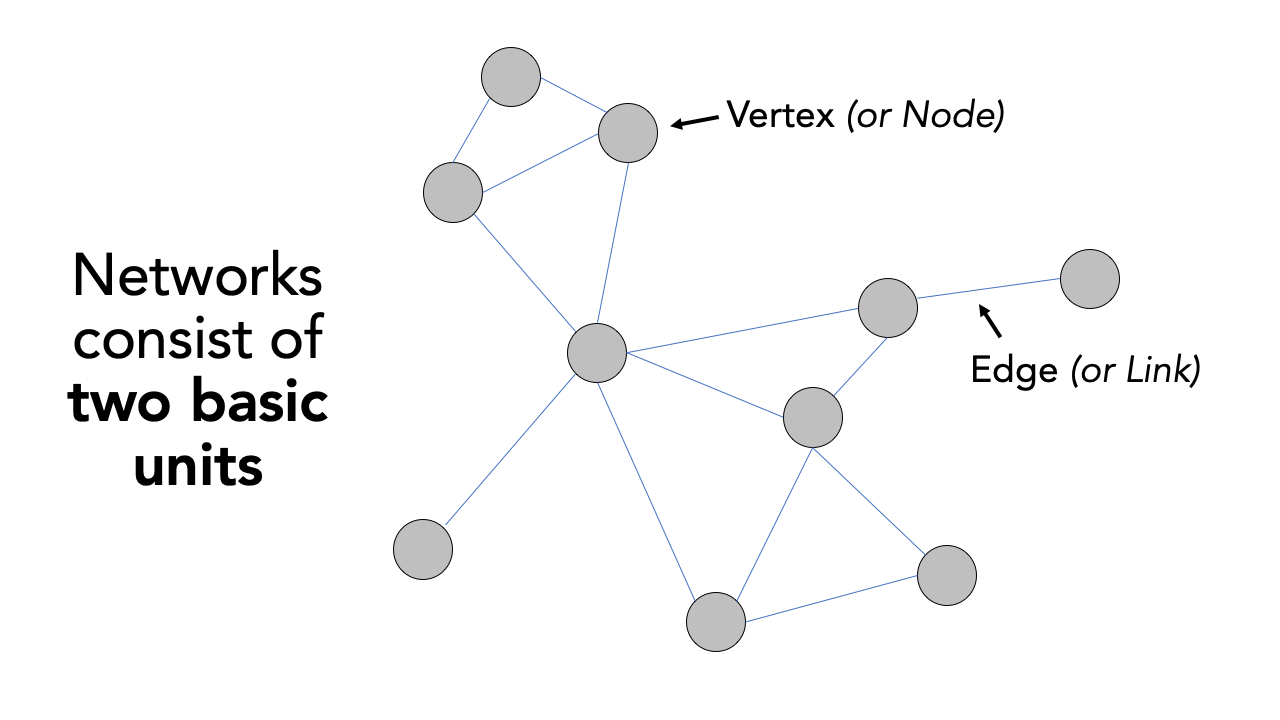
\includegraphics[width=4.27in,height=\textheight]{images/w08/network-graph.png}

}

\caption{\label{fig-ntx-network-graph-example}Visualising networks with
vertices and edges.}

\end{figure}

\hypertarget{accessibility-in-portsmouth}{%
\subsection{Accessibility in
Portsmouth}\label{accessibility-in-portsmouth}}

For this week's practical, we will be using Portsmouth in the UK as our
area of interest for our analysis. One prominent topic within the city
is the issue of public health and childhood obesity. According to
figures released in March 2020 by Public Health England, more than one
in three school pupils are overweight or obese by the time they finish
primary school within the city; this is much higher than the national
average of one in four. One potential contributor to the health crisis
is the ease and availability of fast-food outlets in the city. In the
following, we will measure the accessibility of fast-food outlets within
specific walking distances of all school in Portsmouth starting at 400m,
then 800m and finally a 1km walking distance. We will then aggregate
these results to Lower Super Output Areas (LSOA) and overlay these
results with some socio-economic variables.

To execute this analysis, we will need to first calculate the distances
between our schools and fast-food outlets. This involves calculating the
shortest distance a child would walk between a school and a fast-food
outlet, using roads or streets. We will use the \texttt{dodgr} R package
to conduct this transport network analysis.

\begin{tcolorbox}[enhanced jigsaw, rightrule=.15mm, colback=white, opacityback=0, opacitybacktitle=0.6, coltitle=black, colbacktitle=quarto-callout-note-color!10!white, breakable, arc=.35mm, title=\textcolor{quarto-callout-note-color}{\faInfo}\hspace{0.5em}{Note}, left=2mm, leftrule=.75mm, bottomtitle=1mm, toprule=.15mm, bottomrule=.15mm, colframe=quarto-callout-note-color-frame, toptitle=1mm, titlerule=0mm]

All calculations within the \texttt{dodgr} library currently need to be
run in WGS84/4236. This is why we will not transform the CRS of our data
in this practical.

\end{tcolorbox}

\hypertarget{loading-data-ntx}{%
\subsection{Acquiring network data}\label{loading-data-ntx}}

The first dataset we need to download will help with the visualisation
of our results: boundary data that contains an outline of Portsmouth.

\begin{longtable}[]{@{}
  >{\raggedright\arraybackslash}p{(\columnwidth - 4\tabcolsep) * \real{0.3333}}
  >{\raggedright\arraybackslash}p{(\columnwidth - 4\tabcolsep) * \real{0.3333}}
  >{\raggedright\arraybackslash}p{(\columnwidth - 4\tabcolsep) * \real{0.3333}}@{}}
\toprule\noalign{}
\begin{minipage}[b]{\linewidth}\raggedright
File
\end{minipage} & \begin{minipage}[b]{\linewidth}\raggedright
File Type
\end{minipage} & \begin{minipage}[b]{\linewidth}\raggedright
Link
\end{minipage} \\
\midrule\noalign{}
\endhead
\bottomrule\noalign{}
\endlastfoot
Major towns and cities boundaries 2015 & \texttt{shp} &
\href{https://github.com/jtvandijk/GEOG0114/tree/master/data/zip/major_towns.zip}{Download} \\
\end{longtable}

We can now load the required libraries as well as the major towns and
cities boundaries \texttt{shapefile}.

\begin{codelisting}

\caption{\texttt{R code}}

\begin{Shaded}
\begin{Highlighting}[]
\CommentTok{\# libraries}
\FunctionTok{library}\NormalTok{(tidyverse)}
\FunctionTok{library}\NormalTok{(sf)}
\FunctionTok{library}\NormalTok{(tmap)}
\FunctionTok{library}\NormalTok{(osmdata)}
\FunctionTok{library}\NormalTok{(dodgr)}

\CommentTok{\# load major towns and cities, filter Portsmouth}
\NormalTok{portsmouth\_city }\OtherTok{\textless{}{-}} \FunctionTok{st\_read}\NormalTok{(}\StringTok{"data/outline/Major\_Towns\_and\_Cities\_\_December\_2015\_\_Boundaries.shp"}\NormalTok{,}
    \AttributeTok{stringsAsFactors =} \ConstantTok{FALSE}\NormalTok{) }\SpecialCharTok{\%\textgreater{}\%}
    \FunctionTok{filter}\NormalTok{(tcity15nm }\SpecialCharTok{==} \StringTok{"Portsmouth"}\NormalTok{)}
\end{Highlighting}
\end{Shaded}

\end{codelisting}

\begin{verbatim}
Reading layer `Major_Towns_and_Cities__December_2015__Boundaries' from data source `/Users/justinvandijk/Library/CloudStorage/Dropbox/UCL/Web/jtvandijk.github.io/GEOG0114Q/data/outline/Major_Towns_and_Cities__December_2015__Boundaries.shp' 
  using driver `ESRI Shapefile'
Simple feature collection with 112 features and 5 fields
Geometry type: MULTIPOLYGON
Dimension:     XY
Bounding box:  xmin: -4.204842 ymin: 50.34101 xmax: 1.378014 ymax: 55.03117
Geodetic CRS:  WGS 84
\end{verbatim}

To create our network and Origin-Destination dataset, we will need data
on schools, fast-food outlets, and a streetnetwork. Today we will be
using \href{https://www.openstreetmap.org}{OpenStreetMap} for this. If
you have never come across OpenStreetMap (OSM) before, it is a free
editable map of the world.

\begin{tcolorbox}[enhanced jigsaw, rightrule=.15mm, colback=white, opacityback=0, opacitybacktitle=0.6, coltitle=black, colbacktitle=quarto-callout-note-color!10!white, breakable, arc=.35mm, title=\textcolor{quarto-callout-note-color}{\faInfo}\hspace{0.5em}{Note}, left=2mm, leftrule=.75mm, bottomtitle=1mm, toprule=.15mm, bottomrule=.15mm, colframe=quarto-callout-note-color-frame, toptitle=1mm, titlerule=0mm]

OpenStreetMap's spatial coverage is still unequal across the world -
plus, as you will find if you use the data, the accuracy and quality of
the data can often be quite questionable or simply missing attribute
details that we would like to have, e.g.~types of roads and their speed
limits, to complete specific types of spatial analysis.

\end{tcolorbox}

Whilst there are
\href{https://wiki.openstreetmap.org/wiki/Downloading_data}{various
approaches} to downloading data from OpenStreetMap, we will use the
\texttt{osmdata} library to directly extract our required OpenStreetMap
(OSM) data into a variable. The \texttt{osmdata} library grants access
within R to the \href{https://overpass-turbo.eu/}{Overpass API} that
allows us to run queries on OSM data and then import the data as spatial
objects. These queries are at the heart of these data downloads.

We will go ahead and start with downloading and extracting our road
network data. To OSM data using the \texttt{osmdata} library, we can use
the \texttt{add\_osm\_feature()} function. To use the function, we need
to provided it with either a \emph{bounding box} of our area of interest
(AOI) or a set of points, from which the function will create its own
bounding box. You can find out more about this and details on how to
construct your own queries in the
\href{https://cran.r-project.org/web/packages/osmdata/vignettes/osmdata.html}{data
vignette}.

To use the library (and API), we need to know how to write and run a
query, which requires identifying the \texttt{key} and \texttt{value}
that we need within our query to select the correct data. Essentially
every map element (whether a point, line or polygon) in OSM is
\textbf{tagged} with different attribute data. These \texttt{keys} and
\texttt{values} are used in our queries to extract only map elements of
that feature type - to find out how a feature is tagged in OSM is simply
a case of \href{https://wiki.openstreetmap.org/wiki/Tags}{reading
through the OSM documentation} and becoming familiar with their keys and
values.

To download our road network dataset, we first define a variable to
store our bounding box coordinates, \texttt{p\_bbox()}. We then use this
within our OSM query to extract specific types of road segments within
that bounding box - the results of our query are then stored in an
\texttt{osmdata} object. We will select all OSM features with the
\texttt{highway} tag that are likely to be used by pedestrians (e.g.~not
\texttt{motorways}).

\begin{codelisting}

\caption{\texttt{R code}}

\begin{Shaded}
\begin{Highlighting}[]
\CommentTok{\# define our bbox coordinates for Portsmouth}
\NormalTok{p\_bbox }\OtherTok{\textless{}{-}} \FunctionTok{c}\NormalTok{(}\SpecialCharTok{{-}}\FloatTok{1.113197}\NormalTok{, }\FloatTok{50.775781}\NormalTok{, }\SpecialCharTok{{-}}\FloatTok{1.026508}\NormalTok{, }\FloatTok{50.859941}\NormalTok{)}

\CommentTok{\# pass bounding box coordinates into the OverPassQuery (opq) function only}
\CommentTok{\# download features that are not classified as motorway}
\NormalTok{osmdata }\OtherTok{\textless{}{-}} \FunctionTok{opq}\NormalTok{(}\AttributeTok{bbox =}\NormalTok{ p\_bbox) }\SpecialCharTok{\%\textgreater{}\%}
    \FunctionTok{add\_osm\_feature}\NormalTok{(}\AttributeTok{key =} \StringTok{"highway"}\NormalTok{, }\AttributeTok{value =} \FunctionTok{c}\NormalTok{(}\StringTok{"primary"}\NormalTok{, }\StringTok{"secondary"}\NormalTok{, }\StringTok{"tertiary"}\NormalTok{,}
        \StringTok{"residential"}\NormalTok{, }\StringTok{"path"}\NormalTok{, }\StringTok{"footway"}\NormalTok{, }\StringTok{"unclassified"}\NormalTok{, }\StringTok{"living\_street"}\NormalTok{, }\StringTok{"pedestrian"}\NormalTok{)) }\SpecialCharTok{\%\textgreater{}\%}
    \FunctionTok{osmdata\_sf}\NormalTok{()}
\end{Highlighting}
\end{Shaded}

\end{codelisting}

\begin{tcolorbox}[enhanced jigsaw, rightrule=.15mm, colback=white, opacityback=0, opacitybacktitle=0.6, coltitle=black, colbacktitle=quarto-callout-note-color!10!white, breakable, arc=.35mm, title=\textcolor{quarto-callout-note-color}{\faInfo}\hspace{0.5em}{Note}, left=2mm, leftrule=.75mm, bottomtitle=1mm, toprule=.15mm, bottomrule=.15mm, colframe=quarto-callout-note-color-frame, toptitle=1mm, titlerule=0mm]

In some instances the OSM query will return an error, especially when
several people from the same location are executing the exact same
query. If this happens, you can just read through the instructions and
download a prepared copy of the data that contains \textbf{all} required
OSM Portsmouth data instead:
\href{https://github.com/jtvandijk/GEOG0114/tree/master/data/zip/osm_portmouth.zip}{{[}Link{]}}.

You can load these downloaded data as follows into R:

\begin{codelisting}[H]

\caption{\texttt{R code}}

\begin{Shaded}
\begin{Highlighting}[]
\FunctionTok{load}\NormalTok{(}\StringTok{"../path/to/file/ports\_ff.RData"}\NormalTok{)}
\FunctionTok{load}\NormalTok{(}\StringTok{"../path/to/file/ports\_roads\_edges.RData"}\NormalTok{)}
\FunctionTok{load}\NormalTok{(}\StringTok{"../path/to/file/ports\_schools.RData"}\NormalTok{)}
\end{Highlighting}
\end{Shaded}

\end{codelisting}

After loading your data, you can continue with the analysis in the
\protect\hyperlink{osm}{Measuring Accessiblity} section below, starting
with the creation of a network graph with the `foot weighting' profile.

\end{tcolorbox}

The \texttt{osmdata} object contains the bounding box of your query, a
time-stamp of the query, and then the spatial data as
\texttt{osm\_points}, \texttt{osm\_lines}, \texttt{osm\_multilines} and
\texttt{osm\_polgyons} (which are listed with their respective fields
also detailed). Some of the spatial features maybe empty, depending on
what you asked your query to return. Our next step therefore is to
extract our spatial data from our \texttt{osmdata} object to create our
road network data set. This is in fact incredibly easy, using the
traditional \texttt{\$} R approach to access these spatial features from
our object.

Deciding what to extract is probably the more complicated aspect of this
- mainly as you need to understand how to represent your road network,
and this will usually be determined by the library/functions you will be
using it within. Today, we want to extract the \textbf{edges} of the
network, i.e.~the lines that represent the roads, as well as the
\textbf{nodes} of the network, i.e.~the points that represent the
locations at which the roads start, end, or intersect. For our points,
we will only keep the \texttt{osm\_id} data field, just in case we need
to refer to this later. For our lines, we will keep a little more
information that we might want to use within our transport network
analysis, including the type of road, the maximum speed, and whether the
road is one-way or not.

\begin{codelisting}

\caption{\texttt{R code}}

\begin{Shaded}
\begin{Highlighting}[]
\CommentTok{\# extract the \textasciigrave{}p\textasciigrave{}oints, with their osm\_id.}
\NormalTok{ports\_roads\_nodes }\OtherTok{\textless{}{-}}\NormalTok{ osmdata}\SpecialCharTok{$}\NormalTok{osm\_points[, }\StringTok{"osm\_id"}\NormalTok{]}

\CommentTok{\# extract the lines, with their osm\_id, name, type of highway, max speed and}
\CommentTok{\# oneway attributes}
\NormalTok{ports\_roads\_edges }\OtherTok{\textless{}{-}}\NormalTok{ osmdata}\SpecialCharTok{$}\NormalTok{osm\_lines[, }\FunctionTok{c}\NormalTok{(}\StringTok{"osm\_id"}\NormalTok{, }\StringTok{"name"}\NormalTok{, }\StringTok{"highway"}\NormalTok{, }\StringTok{"maxspeed"}\NormalTok{,}
    \StringTok{"oneway"}\NormalTok{)]}
\end{Highlighting}
\end{Shaded}

\end{codelisting}

To check our data set, we can quickly plot the edges of our road network
using the \texttt{plot()} function:

\begin{codelisting}

\caption{\texttt{R code}}

\begin{Shaded}
\begin{Highlighting}[]
\CommentTok{\# inspect}
\FunctionTok{plot}\NormalTok{(ports\_roads\_edges, }\AttributeTok{max.plot =} \DecValTok{1}\NormalTok{)}
\end{Highlighting}
\end{Shaded}

\end{codelisting}

\begin{figure}[H]

{\centering 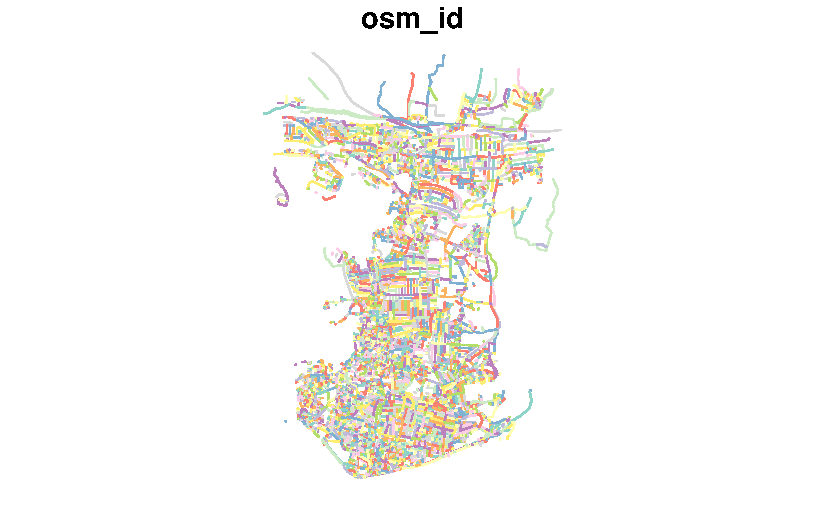
\includegraphics{02-network_files/figure-pdf/fig-ntx-network-plot-1.pdf}

}

\caption{\label{fig-ntx-network-plot}OSM road network}

\end{figure}

Because we are focusing on walking, we will overwrite the
\texttt{oneway} variable by suggesting that none of the road segments
are restricted to one-way traffic which may affect our analysis as well
as the general connectivity of the network.

\begin{codelisting}

\caption{\texttt{R code}}

\begin{Shaded}
\begin{Highlighting}[]
\CommentTok{\# overwrite one{-}way default}
\NormalTok{ports\_roads\_edges}\SpecialCharTok{$}\NormalTok{oneway }\OtherTok{\textless{}{-}} \StringTok{"no"}
\end{Highlighting}
\end{Shaded}

\end{codelisting}

Now we have the network edges, we can turn this into a
graph-representation that allows for the calculation of network-based
accessibility statistics.

\hypertarget{osm}{%
\subsection{Measuring accessibility}\label{osm}}

Before we can construct our full network graph for the purpose of
accessibility analysis, we need to also provide our \textbf{Origin} and
\textbf{Destination} points, i.e.~the data points we wish to calculate
the distances between. According to the \texttt{dodgr} documentation,
these points need to be in either a vector or matrix format, containing
the two coordinates for each point for the origins and for the
destinations.

As for our Portsmouth scenario we are interested in calculating the
shortest distances between schools and fast-food outlets, we need to try
and download these datasets - again we will turn to OpenStreetMap.
Following a similar structure to our query above, we will use our
knowledge of OpenStreetMap \texttt{keys} and \texttt{values} to extract
the points of Origins (schools) and Destinations (fast-food outlets) we
are interested in:

\begin{codelisting}

\caption{\texttt{R code}}

\begin{Shaded}
\begin{Highlighting}[]
\CommentTok{\# download schools from OSM}
\NormalTok{schools }\OtherTok{\textless{}{-}} \FunctionTok{opq}\NormalTok{(}\AttributeTok{bbox =}\NormalTok{ p\_bbox) }\SpecialCharTok{\%\textgreater{}\%}
    \FunctionTok{add\_osm\_feature}\NormalTok{(}\AttributeTok{key =} \StringTok{"amenity"}\NormalTok{, }\AttributeTok{value =} \StringTok{"school"}\NormalTok{) }\SpecialCharTok{\%\textgreater{}\%}
    \FunctionTok{osmdata\_sf}\NormalTok{()}

\CommentTok{\# download fast{-}food outlets}
\NormalTok{ff\_outlets }\OtherTok{\textless{}{-}} \FunctionTok{opq}\NormalTok{(}\AttributeTok{bbox =}\NormalTok{ p\_bbox) }\SpecialCharTok{\%\textgreater{}\%}
    \FunctionTok{add\_osm\_feature}\NormalTok{(}\AttributeTok{key =} \StringTok{"amenity"}\NormalTok{, }\AttributeTok{value =} \StringTok{"fast\_food"}\NormalTok{) }\SpecialCharTok{\%\textgreater{}\%}
    \FunctionTok{osmdata\_sf}\NormalTok{()}
\end{Highlighting}
\end{Shaded}

\end{codelisting}

We also need to then extract the relevant data from the \texttt{osmdata}
object:

\begin{codelisting}

\caption{\texttt{R code}}

\begin{Shaded}
\begin{Highlighting}[]
\CommentTok{\# extract school points}
\NormalTok{ports\_schools }\OtherTok{\textless{}{-}}\NormalTok{ schools}\SpecialCharTok{$}\NormalTok{osm\_points[, }\FunctionTok{c}\NormalTok{(}\StringTok{"osm\_id"}\NormalTok{, }\StringTok{"name"}\NormalTok{)]}

\CommentTok{\# extract fast{-}food outlet points}
\NormalTok{ports\_ff }\OtherTok{\textless{}{-}}\NormalTok{ ff\_outlets}\SpecialCharTok{$}\NormalTok{osm\_points[, }\FunctionTok{c}\NormalTok{(}\StringTok{"osm\_id"}\NormalTok{, }\StringTok{"name"}\NormalTok{)]}
\end{Highlighting}
\end{Shaded}

\end{codelisting}

We now have our road network data and our Origin-Destination (OD) points
in place and we can now move to construct our network graph and run our
transport network analysis.

\begin{tcolorbox}[enhanced jigsaw, rightrule=.15mm, colback=white, opacityback=0, opacitybacktitle=0.6, coltitle=black, colbacktitle=quarto-callout-note-color!10!white, breakable, arc=.35mm, title=\textcolor{quarto-callout-note-color}{\faInfo}\hspace{0.5em}{Note}, left=2mm, leftrule=.75mm, bottomtitle=1mm, toprule=.15mm, bottomrule=.15mm, colframe=quarto-callout-note-color-frame, toptitle=1mm, titlerule=0mm]

In this analysis, we are highly reliant on the use of OpenStreetMap to
provide data for both our Origins and Destinations. Whilst in the UK OSM
provides substantial coverage, its quality is not always guaranteed. As
a result, to improve on our current methodology in future analysis, we
should investigate into a more official school data set or at least
validate the number of schools against City Council records. The same
applies to our fast-food outlets.

\end{tcolorbox}

With any network analysis, the main data structure is a \textbf{graph},
constructed by our nodes and edges. To create a graph for use within
\texttt{dodgr}, we pass our \texttt{ports\_roads\_edges()} into the
\texttt{weight\_streetnet()} function. The \texttt{dodgr} library also
contains weighting profiles, that you can customise, for use within your
network analysis. These weighting profiles contain weights based on the
type of road, determined by the type of transportation the profile aims
to model. Here we will use the weighting profile \textbf{foot}, as we
are looking to model walking accessibility.

\begin{codelisting}

\caption{\texttt{R code}}

\begin{Shaded}
\begin{Highlighting}[]
\CommentTok{\# create network graph with the foot weighting profile}
\NormalTok{graph }\OtherTok{\textless{}{-}} \FunctionTok{weight\_streetnet}\NormalTok{(ports\_roads\_edges, }\AttributeTok{wt\_profile =} \StringTok{"foot"}\NormalTok{)}
\end{Highlighting}
\end{Shaded}

\end{codelisting}

Once we have our graph, we can then use this to calculate our network
distances between our OD points. One thing to keep in mind is that
potentially not all individual components in the network that we
extracted are connected, for instance, because the bounding box cut off
the access road of a
\href{https://en.wikipedia.org/wiki/Dead_end_(street)}{cul-de-sac}. To
make sure that our entire extracted network is connected, we now extract
the \textbf{largest connected component} of the graph. You can use
\texttt{table(graph\$component)} to examine the sizes of all individual
subgraphs. You will notice that most subgraphs consist of a very small
number of edges.

\begin{tcolorbox}[enhanced jigsaw, rightrule=.15mm, colback=white, opacityback=0, opacitybacktitle=0.6, coltitle=black, colbacktitle=quarto-callout-note-color!10!white, breakable, arc=.35mm, title=\textcolor{quarto-callout-note-color}{\faInfo}\hspace{0.5em}{Note}, left=2mm, leftrule=.75mm, bottomtitle=1mm, toprule=.15mm, bottomrule=.15mm, colframe=quarto-callout-note-color-frame, toptitle=1mm, titlerule=0mm]

The \texttt{dodgr} package documentation explains that components are
numbered in order of decreasing size, with \texttt{\$component\ =\ 1}
always denoting the largest component. Always inspect the resulting
subgraph to make sure that its coverage is adequate for analysis.

\end{tcolorbox}

\begin{codelisting}

\caption{\texttt{R code}}

\begin{Shaded}
\begin{Highlighting}[]
\CommentTok{\# extract the largest connected graph component}
\NormalTok{graph\_connected }\OtherTok{\textless{}{-}}\NormalTok{ graph[graph}\SpecialCharTok{$}\NormalTok{component }\SpecialCharTok{==} \DecValTok{1}\NormalTok{, ]}

\CommentTok{\# inspect number of remaining road segments}
\FunctionTok{nrow}\NormalTok{(graph\_connected)}
\end{Highlighting}
\end{Shaded}

\end{codelisting}

\begin{verbatim}
[1] 56364
\end{verbatim}

\begin{Shaded}
\begin{Highlighting}[]
\CommentTok{\# inspect}
\FunctionTok{plot}\NormalTok{(}\FunctionTok{dodgr\_to\_sf}\NormalTok{(graph\_connected), }\AttributeTok{max.plot =} \DecValTok{1}\NormalTok{)}
\end{Highlighting}
\end{Shaded}

\begin{figure}[H]

{\centering 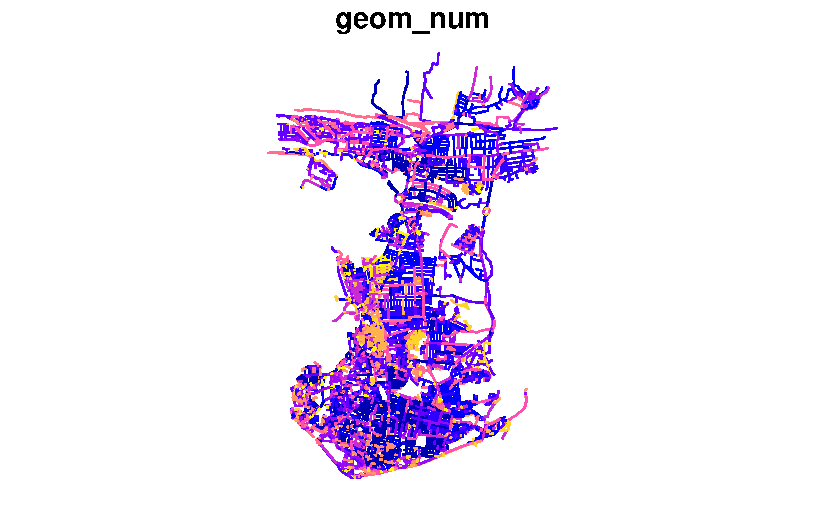
\includegraphics{02-network_files/figure-pdf/fig-ntx-extract-largest-graph-1.pdf}

}

\caption{\label{fig-ntx-extract-largest-graph}Largest graph component}

\end{figure}

\begin{tcolorbox}[enhanced jigsaw, rightrule=.15mm, colback=white, opacityback=0, opacitybacktitle=0.6, coltitle=black, colbacktitle=quarto-callout-warning-color!10!white, breakable, arc=.35mm, title=\textcolor{quarto-callout-warning-color}{\faExclamationTriangle}\hspace{0.5em}{Warning}, left=2mm, leftrule=.75mm, bottomtitle=1mm, toprule=.15mm, bottomrule=.15mm, colframe=quarto-callout-warning-color-frame, toptitle=1mm, titlerule=0mm]

OpenStreetMap is a living dataset, meaning that changes are made on a
continuous basis; as such it may very well possible that the number of
remaining road segments as shown above may be slighlty different when
you run this analysis.

\end{tcolorbox}

Now we have our connected subgraph, will can use the
\texttt{dodgr\_distances()} function to calculate the network distances
between every possible Origin and Destination. In the
\texttt{dodgr\_distances()} function, we first pass our \texttt{graph},
then our Origin points (schools), in the \texttt{from} argument, and
then our Destination points (fast-food outlets), in the \texttt{to}
argument. One thing to note is our addition of the
\texttt{st\_coordinates()} function as we pass our two point data sets
within the \texttt{from} and \texttt{to} functions as we need to
supplement our Origins and Destinations in a matrix format. For all
Origins and Destinations, \texttt{dodgr\_distances()} will map the
points to the \textbf{closest network points}, and return corresponding
shortest-path distances.

\begin{codelisting}

\caption{\texttt{R code}}

\begin{Shaded}
\begin{Highlighting}[]
\CommentTok{\# create a distance matrix between schools and fast{-}food stores}
\NormalTok{sch\_to\_ff\_calc }\OtherTok{\textless{}{-}} \FunctionTok{dodgr\_distances}\NormalTok{(graph\_connected, }\AttributeTok{from =} \FunctionTok{st\_coordinates}\NormalTok{(ports\_schools),}
    \AttributeTok{to =} \FunctionTok{st\_coordinates}\NormalTok{(ports\_ff), }\AttributeTok{shortest =} \ConstantTok{TRUE}\NormalTok{, }\AttributeTok{pairwise =} \ConstantTok{FALSE}\NormalTok{, }\AttributeTok{quiet =} \ConstantTok{FALSE}\NormalTok{)}
\end{Highlighting}
\end{Shaded}

\end{codelisting}

The result of this computation is a distance-matrix that contains the
network distances between all Origins (i.e.~schools) and all
Destinations (i.e.~fast-food outlets). Let's inspect the first row of
our output. Do you understand what the values mean?

\begin{codelisting}

\caption{\texttt{R code}}

\begin{Shaded}
\begin{Highlighting}[]
\CommentTok{\# inspect}
\FunctionTok{head}\NormalTok{(sch\_to\_ff\_calc, }\AttributeTok{n =} \DecValTok{1}\NormalTok{)}
\end{Highlighting}
\end{Shaded}

\end{codelisting}

\begin{verbatim}
         1        2        3       4        5        6        7        8
1 4000.016 2090.485 6549.779 9356.08 10903.62 2231.919 11845.44 2292.263
         9       10       11       12       13       14       15       16
1 1676.805 1680.043 1697.416 1676.805 2090.485 2090.485 2060.898 4000.016
        17       18       19      20       21       22       23       24
1 2324.454 4000.016 4000.016 3338.83 1700.179 581.0582 7277.651 3610.322
        25       26       27       28       29       30       31       32
1 1359.146 3321.374 340.8823 1102.226 10796.81 2963.157 2720.491 3508.267
        33       34       35       36       37       38       39       40
1 2330.386 2818.121 2920.565 2920.565 736.0556 3399.756 844.6083 6231.901
        41       42       43       44       45       46       47       48
1 3394.397 9171.192 9372.628 9238.263 9481.949 1629.029 3525.506 2400.918
        49       50       51       52       53       54       55       56
1 7173.413 8978.739 9403.034 9329.926 6483.465 6483.465 6470.802 6470.802
        57       58       59       60       61       62       63       64
1 804.5849 763.0434 2526.807 1067.907 1010.408 1010.408 1967.697 1418.767
        65       66      67       68       69       70       71       72
1 2818.121 1245.823 2157.02 688.8672 2162.922 2205.285 2119.323 11755.26
        73       74       75       76       77       78       79       80
1 4829.051 2738.124 844.6083 615.1102 788.7212 2586.476 2667.125 728.4882
        81       82       83       84       85       86       87       88
1 11845.44 11845.44 11845.44 11934.59 11934.59 11934.59 11845.44 11845.44
        89       90       91       92       93       94       95       96
1 11845.44 11845.44 11845.44 11845.44 11845.44 11339.91 6545.668 6589.917
        97       98       99      100      101      102      103      104
1 6589.917 6442.566 4000.016 4000.016 4234.432 5929.469 3841.384 581.0582
       105      106      107      108      109      110      111      112
1 597.3575 2654.314 5119.621 5317.048 5058.497 375.2084 926.0127 5058.497
       113     114      115     116      117      118     119      120      121
1 4045.705 753.752 556.5173 713.536 622.6949 597.3575 1225.66 3339.134 3295.758
       122      123      124      125     126      127      128     129
1 5469.038 6670.481 6634.905 6634.905 6626.71 6634.905 6634.905 6626.71
       130      131     132      133      134      135      136      137
1 6670.481 6670.481 6626.71 6670.481 6670.481 6670.481 6670.481 6670.481
       138      139      140      141      142      143      144      145
1 12348.71 9528.601 9528.601 5522.227 9339.459 9339.459 9291.034 8563.944
       146      147      148      149     150      151     152      153
1 9291.034 9339.459 12026.51 12026.51 12033.8 12026.11 9548.47 3586.662
       154      155      156      157      158      159      160      161
1 2300.121 815.5434 3467.049 5708.154 905.8238 905.8238 905.8238 4950.036
       162      163      164      165      166      167      168    169
1 4968.988 858.9023 3216.085 3397.074 11419.74 4879.532 1813.109 9160.3
       170     171      172      173      174      175      176      177
1 1666.407 9599.24 9659.195 4687.627 3177.171 3467.049 3118.594 5973.195
       178      179      180      181      182      183      184      185
1 9633.051 9659.195 5299.098 3966.434 9219.851 6041.409 5972.696 8905.439
       186      187      188      189      190      191      192      193
1 6656.006 5895.308 10772.24 1505.914 4995.748 11489.11 1574.826 5478.182
       194      195      196      197      198      199      200      201
1 1804.091 3107.774 9102.648 4738.493 4968.988 4041.569 13159.31 5478.182
       202      203      204      205      206      207      208      209
1 3295.758 3295.758 556.5173 788.7212 10113.11 5101.577 9633.051 9633.051
       210      211      212      213      214      215      216      217
1 9633.051 9520.773 9520.773 9520.773 9520.773 9633.051 9633.051 6001.071
      218      219      220      221      222      223      224      225
1 5606.02 4718.064 4041.569 4887.462 4885.475 1543.604 1510.665 1559.537
       226      227      228      229      230      231      232      233
1 5317.388 11646.67 4944.579 4949.291 4188.983 3525.506 6046.467 5452.211
       234      235      236      237      238      239      240      241
1 5317.048 5317.048 5317.048 5317.048 5317.048 5317.048 5317.048 4963.868
       242      243      244      245      246      247     248      249
1 6272.114 5376.342 4738.493 5818.335 6634.905 4925.352 11559.4 11584.02
       250      251      252      253      254      255      256      257
1 5058.497 5058.497 5058.497 5058.497 5101.577 5131.313 5101.577 5131.313
       258      259      260      261      262      263      264      265
1 5131.313 5125.567 11845.44 6549.779 6549.779 6529.533 6549.779 6549.779
       266      267      268      269      270      271      272      273
1 6529.533 4808.089 4968.988 11845.44 4774.109 4361.855 1129.672 1302.289
       274      275      276     277      278      279      280      281
1 1302.289 1320.727 3344.664 4341.78 1332.226 1122.057 5297.203 11934.59
       282     283      284      285      286      287      288      289
1 12026.51 3002.79 6483.465 5784.828 3383.088 3166.965 11584.02 2920.565
      290      291      292      293     294      295      296      297
1 1677.06 2312.611 5837.072 5735.345 5737.21 5837.072 5837.072 4958.337
       298     299      300      301     302      303      304      305
1 1128.534 9233.39 2059.118 7701.615 1114.85 1092.164 1092.164 1122.057
       306     307      308      309      310      311      312      313
1 1092.164 4661.76 2205.285 3361.814 2738.453 3026.324 3508.075 3522.959
       314      315      316      317      318      319      320      321
1 3522.959 3610.322 3610.322 3639.371 3377.222 3522.959 2724.716 597.3575
       322     323      324      325     326
1 3532.616 7376.95 7338.052 7338.052 7376.95
\end{verbatim}

Our output shows the calculations for the first school - and the
distances between the school and every fast-food outlet. Because we
manually overwrote the values for all one-way streets as well as that we
extracted the larges connected graph only, we currently should not have
any \texttt{NA} values.

\begin{tcolorbox}[enhanced jigsaw, rightrule=.15mm, colback=white, opacityback=0, opacitybacktitle=0.6, coltitle=black, colbacktitle=quarto-callout-tip-color!10!white, breakable, arc=.35mm, title=\textcolor{quarto-callout-tip-color}{\faLightbulb}\hspace{0.5em}{Tip}, left=2mm, leftrule=.75mm, bottomtitle=1mm, toprule=.15mm, bottomrule=.15mm, colframe=quarto-callout-tip-color-frame, toptitle=1mm, titlerule=0mm]

The
\href{https://cran.r-project.org/web/packages/dodgr/vignettes/dodgr.html\#4_Distance_Matrices:_dodgr_dists()}{\texttt{dodgr}
vignette} notes that a distance matrix obtained from running
\texttt{dodgr\_distances} on \texttt{graph\_connected} should generally
contain no \texttt{NA} values, although some points may still be
effectively unreachable due to one-way connections (or streets). Thus,
routing on the largest connected component of a directed graph ought to
be expected to yield the minimal number of \texttt{NA} values, which may
sometimes be more than zero. Note further that spatial routing points
(expressed as from and/or to arguments) will in this case be mapped to
the nearest vertices of \texttt{graph\_connected}, rather than the
potentially closer nearest points of the full graph.

\end{tcolorbox}

The next step of processing all depends on what you are trying to assess
- here we want to understand which schools have a higher accessibility
of fast-food outlets compared to others, quantified by how many outlets
are within walking distance of specific distances. We will therefore
look to count how many outlets are with walking distance from each
school and store this as a new column within our \texttt{ports\_school}
data frame.

\begin{codelisting}

\caption{\texttt{R code}}

\begin{Shaded}
\begin{Highlighting}[]
\CommentTok{\# fastfood outlets within 400m}
\NormalTok{ports\_schools}\SpecialCharTok{$}\NormalTok{ff\_within\_400m }\OtherTok{\textless{}{-}} \FunctionTok{rowSums}\NormalTok{(sch\_to\_ff\_calc }\SpecialCharTok{\textless{}=} \DecValTok{400}\NormalTok{)}

\CommentTok{\# fastfood outlets within 800m}
\NormalTok{ports\_schools}\SpecialCharTok{$}\NormalTok{ff\_within\_800m }\OtherTok{\textless{}{-}} \FunctionTok{rowSums}\NormalTok{(sch\_to\_ff\_calc }\SpecialCharTok{\textless{}=} \DecValTok{800}\NormalTok{)}

\CommentTok{\# fastfood outlets within 1000m}
\NormalTok{ports\_schools}\SpecialCharTok{$}\NormalTok{ff\_within\_1km }\OtherTok{\textless{}{-}} \FunctionTok{rowSums}\NormalTok{(sch\_to\_ff\_calc }\SpecialCharTok{\textless{}=} \DecValTok{1000}\NormalTok{)}
\end{Highlighting}
\end{Shaded}

\end{codelisting}

\hypertarget{task-ntx}{%
\subsection{Tutorial task}\label{task-ntx}}

Now you have calculated the number of fast-food outlets within specific
distances from every school in Portsmouth, your task is to estimate the
accessibility of fast-food outlets at the LSOA scale and compare this to
the
\href{https://www.gov.uk/government/statistics/english-indices-of-deprivation-2019}{2019
Index of Multiple Deprivation}.

\begin{tcolorbox}[enhanced jigsaw, rightrule=.15mm, colback=white, opacityback=0, opacitybacktitle=0.6, coltitle=black, colbacktitle=quarto-callout-tip-color!10!white, breakable, arc=.35mm, title=\textcolor{quarto-callout-tip-color}{\faLightbulb}\hspace{0.5em}{Tip}, left=2mm, leftrule=.75mm, bottomtitle=1mm, toprule=.15mm, bottomrule=.15mm, colframe=quarto-callout-tip-color-frame, toptitle=1mm, titlerule=0mm]

This skills and steps required for this analysis are not just based on
this week's practical, but you will have to combine all your knowledge
of coding and spatial analysis you have gained over the past weeks.

\end{tcolorbox}

One way of doing this, is by taking some of the following steps:

\begin{itemize}
\tightlist
\item
  Download and extract the 2011 LSOA boundaries of Portsmouth.
\item
  Download the
  \href{https://www.gov.uk/government/statistics/english-indices-of-deprivation-2019}{2019
  Index of Multiple Deprivation} scores.
\item
  Decide on an accessibility measure, such as:

  \begin{itemize}
  \tightlist
  \item
    The average number of fast-food restaurants within \texttt{x} meters
    of a school within each LSOA.
  \item
    The average distance a fast-food restaurant is from a school within
    each LSOA.
  \item
    The (average) shortest distance a fast-food restaurant is from a
    school within each LSOA.
  \item
    The minimum shortest distance a fast-food outlet is from a school
    within each LSOA.
  \end{itemize}
\item
  Create a choropleth map of aggregate accessibility to visualise the
  results.
\item
  Join the 2019 Index of Multiple Deprivation data to your LSOA dataset.
\item
  For each IMD decile, calculate the average for your chosen aggregate
  measure and produce a table.
\end{itemize}

Using your approach what do you think: are fast-food restaurants, on
average, more accessible for students at schools that are located within
LSOAs with a lower IMD decile when compared to students at schools that
are located within LSOAs with a higher IMD decile?

\hypertarget{wm-w10}{%
\section{Want more? {[}Optional{]}}\label{wm-w10}}

We have now conducted some basic accessibility analysis, however, there
is some additional fundamental challenges to consider in the context of
transport network and accessibility analysis:

\begin{enumerate}
\def\labelenumi{\arabic{enumi}.}
\tightlist
\item
  How do the different weight profiles of the \texttt{dodgr} package
  work? How would one go about creating your own weight profile? How
  would using a different weight profiles affect the results of your
  analysis?
\item
  Why do we have unconnected segments in the extracted transport
  network? How would you inspect these unconnected segments? Would they
  need to be connected? If so, how would one do this?
\item
  Why you think all Origins and Destinations are mapped onto the closest
  network points? Is this always the best option? What alternative
  methods could you think of and how would you implement these?
\end{enumerate}

\begin{tcolorbox}[enhanced jigsaw, rightrule=.15mm, colback=white, opacityback=0, opacitybacktitle=0.6, coltitle=black, colbacktitle=quarto-callout-tip-color!10!white, breakable, arc=.35mm, title=\textcolor{quarto-callout-tip-color}{\faLightbulb}\hspace{0.5em}{Tip}, left=2mm, leftrule=.75mm, bottomtitle=1mm, toprule=.15mm, bottomrule=.15mm, colframe=quarto-callout-tip-color-frame, toptitle=1mm, titlerule=0mm]

If you want to take a deepdive into accessibility analysis, there is a
great resource that got published recently:
\href{https://ipeagit.github.io/intro_access_book/}{Introduction to
urban accessibility: a practical guide in R}.

\end{tcolorbox}

\hypertarget{byl-ntx}{%
\section{Before you leave}\label{byl-ntx}}

Having finished this tutorial on transport network analysis and,
hopefully, having been able to independently conduct some further
area-profiling using IMD deciles,
\href{https://www.youtube.com/watch?v=fFw7q-BLxLA}{you have now reached
the end of this week's content}. However, there is some additional
fundamental challenges to consider in the context of transport network
and accessibility analysis:

\begin{enumerate}
\def\labelenumi{\arabic{enumi}.}
\tightlist
\item
  How do the different weight profiles of the \texttt{dodgr} package
  work? How would one go about creating your own weight profile? How
  would using a different weight profiles affect the results of your
  analysis?
\item
  Why do we have unconnected segments in the extracted transport
  network? How would you inspect these unconnected segments? Would they
  need to be connected? If so, how would one do this?
\item
  Why you think all Origins and Destinations are mapped onto the closest
  network points? Is this always the best option? What alternative
  methods could you think of and how would you implement these?
\end{enumerate}



\end{document}
